%%
%% Apresentação do Projeto.tex
%% Projeto Oficinas de Integração 3
%% Created by Leonardo Winter Pereira and Lucas Zimmermann Cordeiro on 10.03.2016
%% Copyright (C). All rights reserved
%%

\documentclass[hyperref={pdfpagelabels=false}]{beamer}

\usepackage[brazil, portuges]{babel} % pacote português brasileiro
\usepackage[utf8]{inputenc} % pacote para acentuação direta
\usepackage{lmodern}
\usetheme{CambridgeUS}
\usepackage{graphicx}
\usepackage[3D]{movie15}
\usepackage{lmodern}
\usepackage{xcolor,colortbl} % para poder utilizar cores em uma tabela
\usepackage{booktabs, tabularx, ltablex, longtable, supertabular} % para poder usar tabelas em múltiplas páginas
\usepackage{multirow} % para poder usar Linhas e Colunas multiplas em tabelas
\usepackage{array, hhline} %mais opcoes para o ambiente tabular
\usepackage{caption, subcaption} % para figuras / subfiguras
\usepackage{eurosym} % para o símbolo do euro
\definecolor{darkRed}{rgb}{0.3, 0.3, 0.3}
\definecolor{lightRed}{rgb}{0.674509803922, 0.674509803922, 0.674509803922}

\title{Dalle Pad \newline O \textit{Gadget} que te transforma em um DJ}
\author{Leonardo Winter Pereira \newline Lucas Zimmermann Cordeiro \newline Luís Felipe Mazzuchetti Ortiz}
\date{\today}

\begin{document}

    \begin{frame}

        \begin{figure}
            
\includegraphics[scale=0.15]{Imagens/Logo01.png}
            %\caption{Dalle Pad - O Gadget que te transforma em um DJ}
        \end{figure}
        \titlepage

    \end{frame}

    \begin{frame}\frametitle{Índice}
        \tableofcontents
    \end{frame}

        \section{Introdução}

            \begin{frame}\frametitle{Introdução}

                \begin{itemize}
                  \item Dalle Pad: O que é?
                  \item Motivação;
                  \item Objetivo.
                        \begin{figure}[H]
                        	\centering
                        	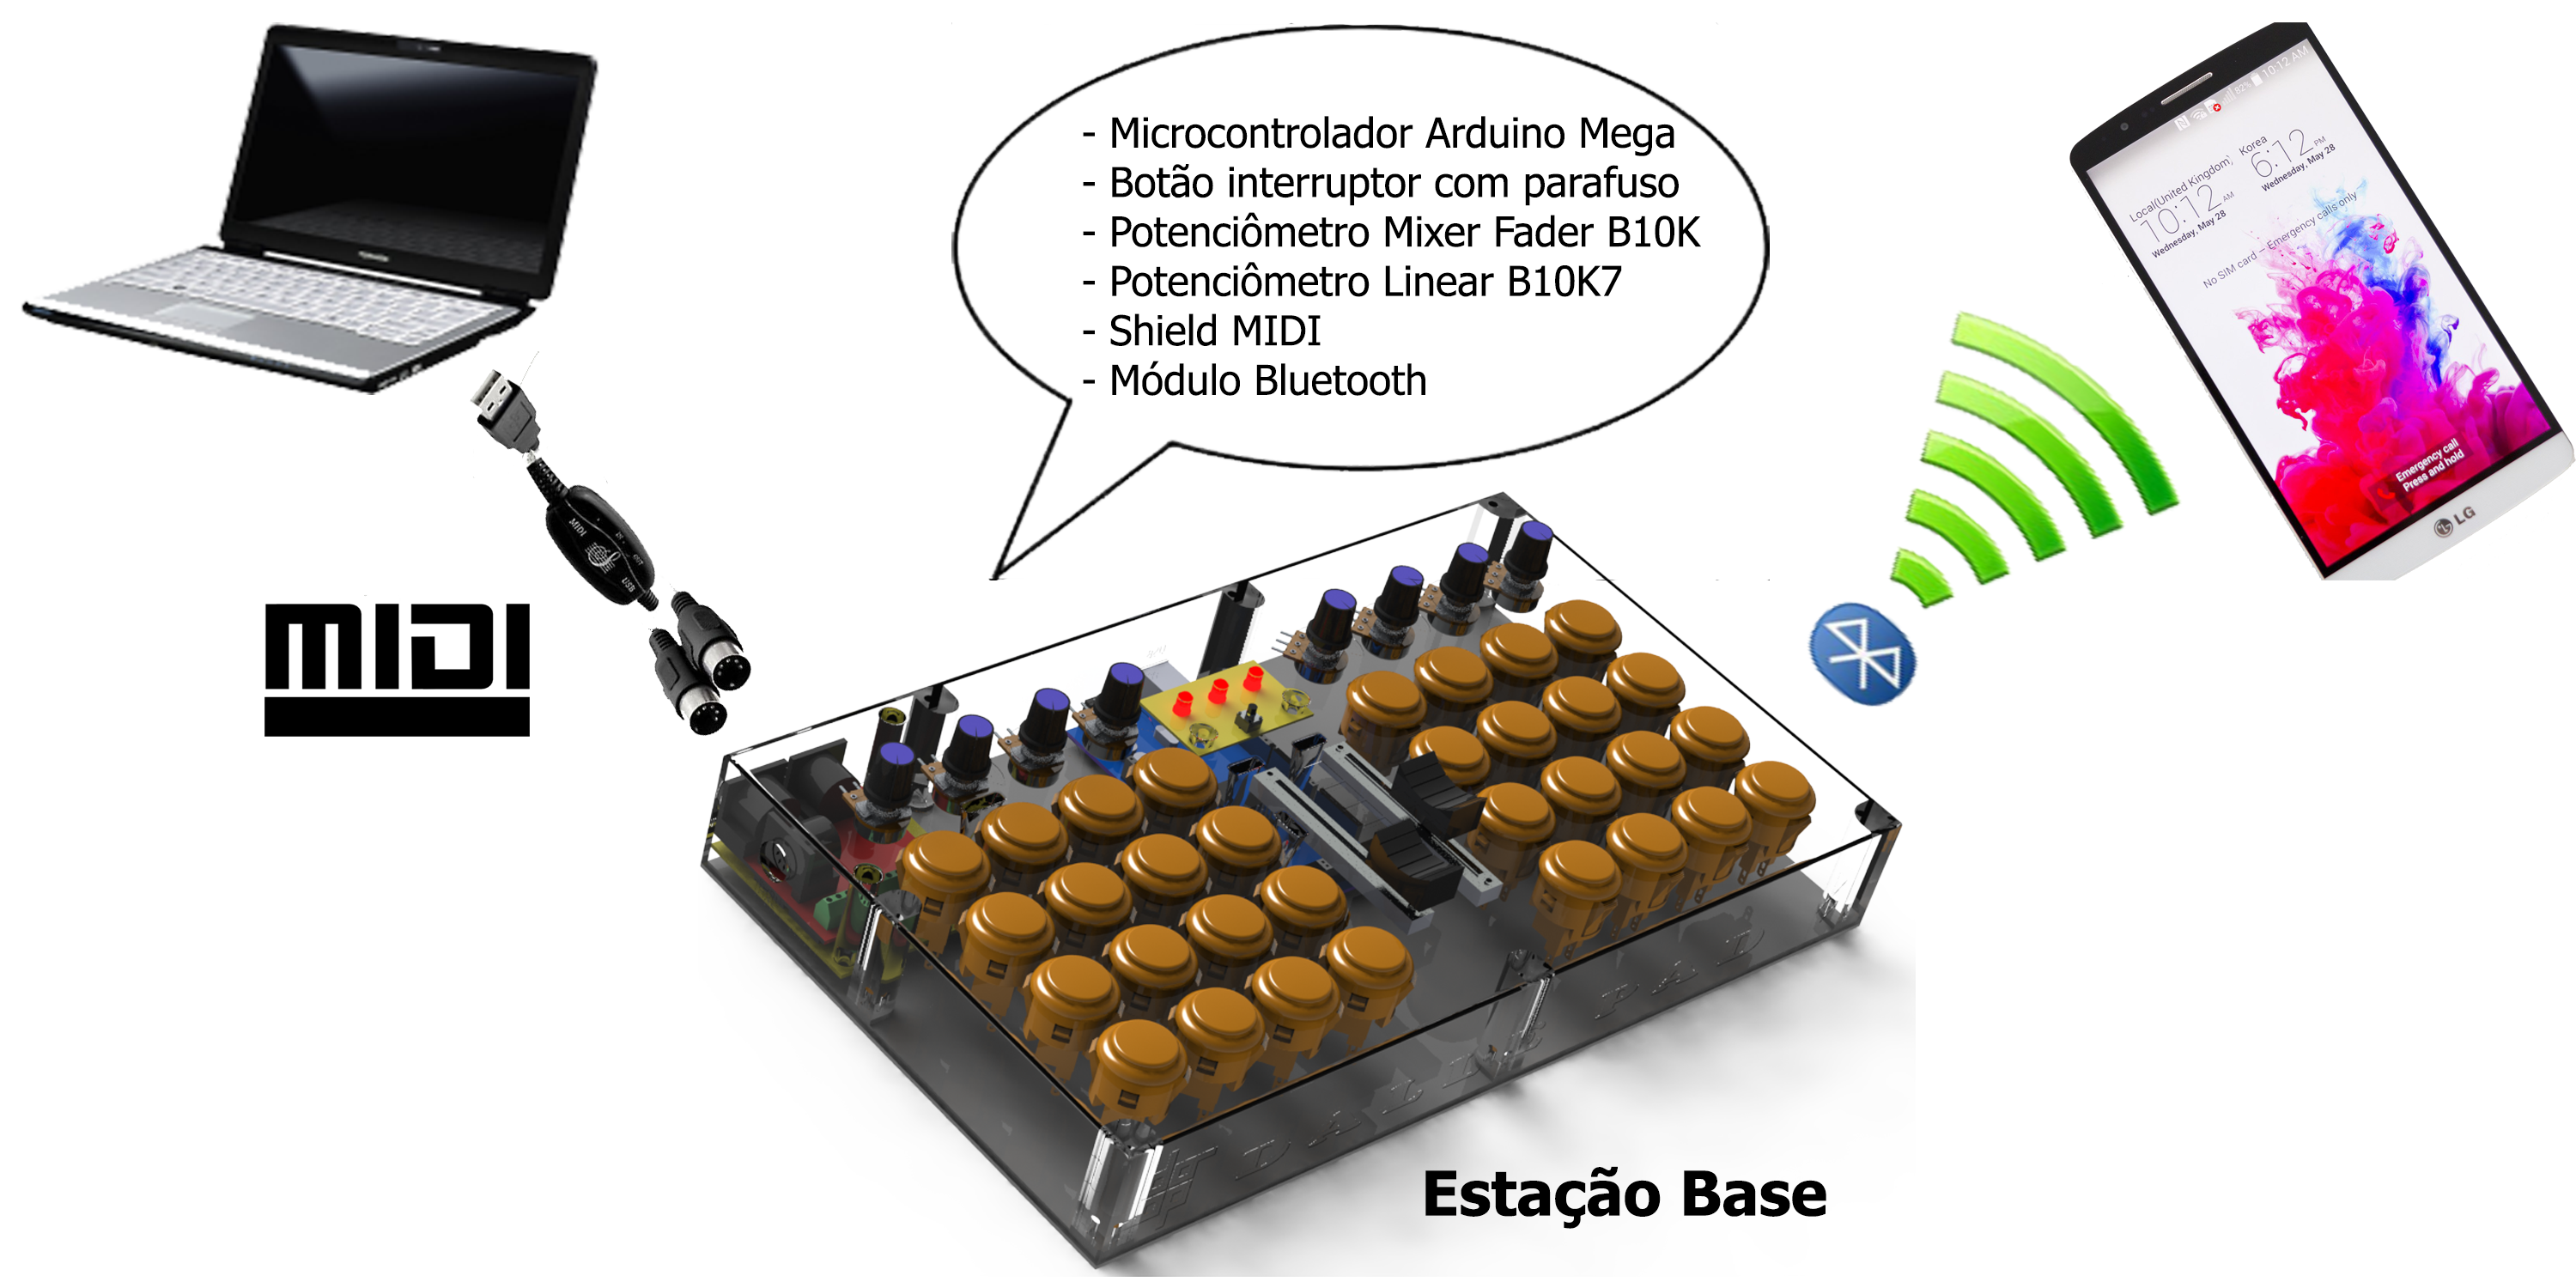
\includegraphics[scale=0.1]{Imagens/imagem-geral-(Fundo-Branco).png}
                        	\caption[Visão Geral do Dalle Pad]{Visão Geral do Dalle Pad}
                        	\label{fig:visao-geral}
                        \end{figure}
                \end{itemize}

            \end{frame}

            \begin{frame}\frametitle{MIDI}

                \begin{itemize}

                  \item O que é?
                        \begin{figure}[H]
                        	\centering
                        	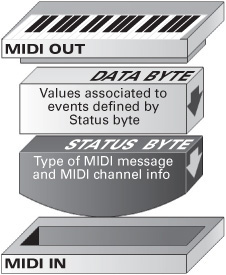
\includegraphics[scale=0.6]{Imagens/Status_and_Data_Bytes.jpg}
                        	\caption[Estrutura de uma mensagem MIDI]{Estrutura de uma mensagem MIDI}
                        	\label{fig:estrutura-midi}
                        \end{figure}
                \end{itemize}

            \end{frame}

            \begin{frame}\frametitle{Requisitos}

                \begin{itemize}
                  \item Requisitos Funcionais
                    \begin{itemize}
                      \item O aplicativo Android, desenvolvido pela equipe, deverá realizar funções básicas, como alterar efeitos e tocá-los através do pressionameto de um botão.
                    \end{itemize}
                  \item Requisitos Não-Funcionais
                    \begin{itemize}
                      \item O sistema embarcado deverá apresentar conexão MIDI com programas terceirizados no computador e conexão \textit{Bluetooth} com o aplicativo Android desenvolvido pela equipe;
                      %\item O invólucro deverá ser de um material que possa ser desenvolvido pela equipe.
                    \end{itemize}
                \end{itemize}

                %\begin{figure}[H]
                %	\centering
                %	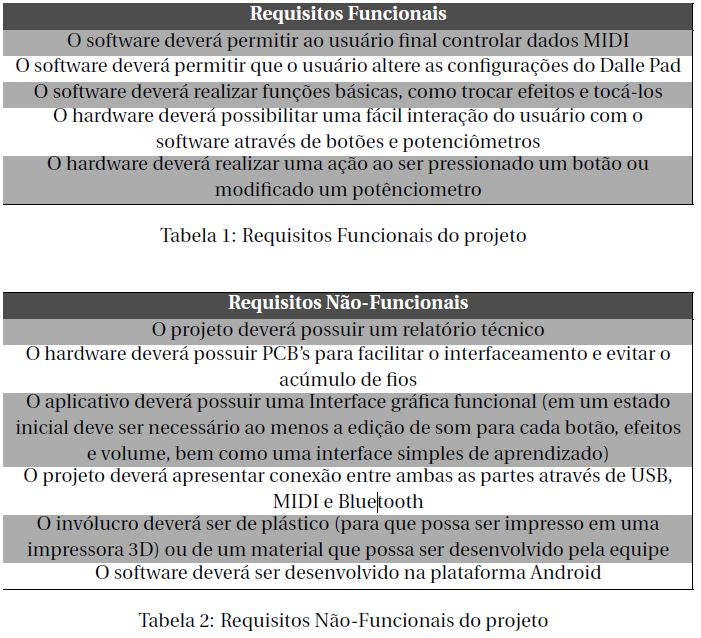
\includegraphics[scale=0.4]{Imagens/requisitos.jpg}
                	%\caption[Visão Geral do Dalle Pad]{Visão Geral do Dalle Pad}
                %	\label{fig:requisitos}
                %\end{figure}

            \end{frame}

            \begin{frame}\frametitle{Conexão MIDI com programa terceirizado}

                \begin{itemize}
                  \item O programa para computador escolhido para testes foi o \textit{Ableton} e não foi desenvolvido pela equipe;
                 \end{itemize}
                        \begin{figure}[H]
                        	\centering
                            \begin{subfigure}[b]{.45\textwidth}
                                \centering
                                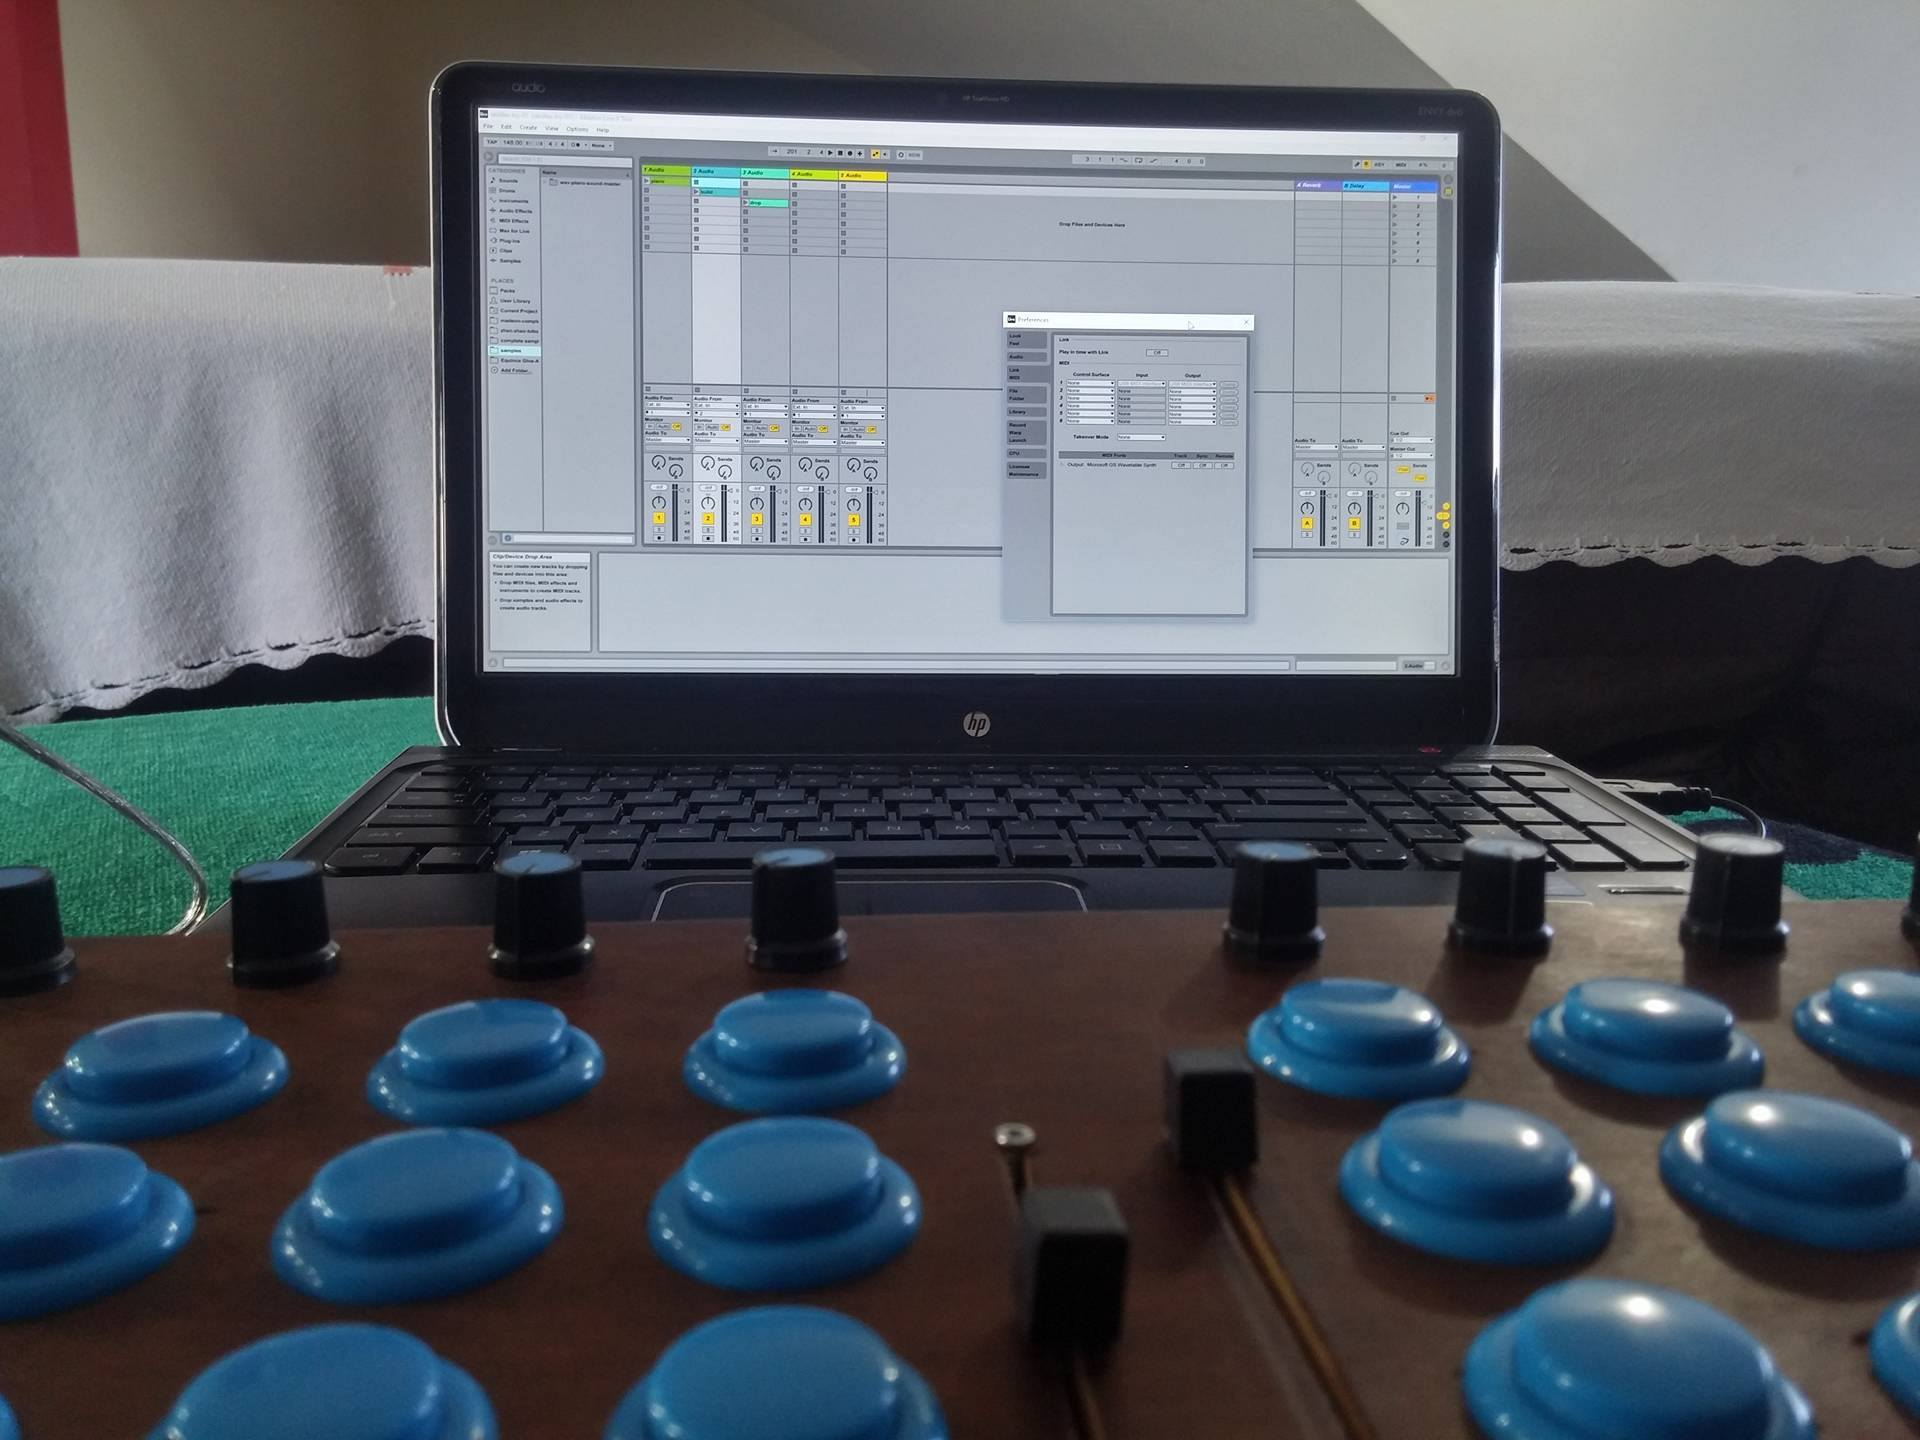
\includegraphics[scale=0.08]{Imagens/ableton1.jpg}
                            	\caption[Dalle pad sem conexão MIDI]{Dalle pad sem conexão MIDI}
                                \label{fig:shield-midi}
                            \end{subfigure} %
                            \begin{subfigure}[b]{.45\textwidth}
                                \centering
                                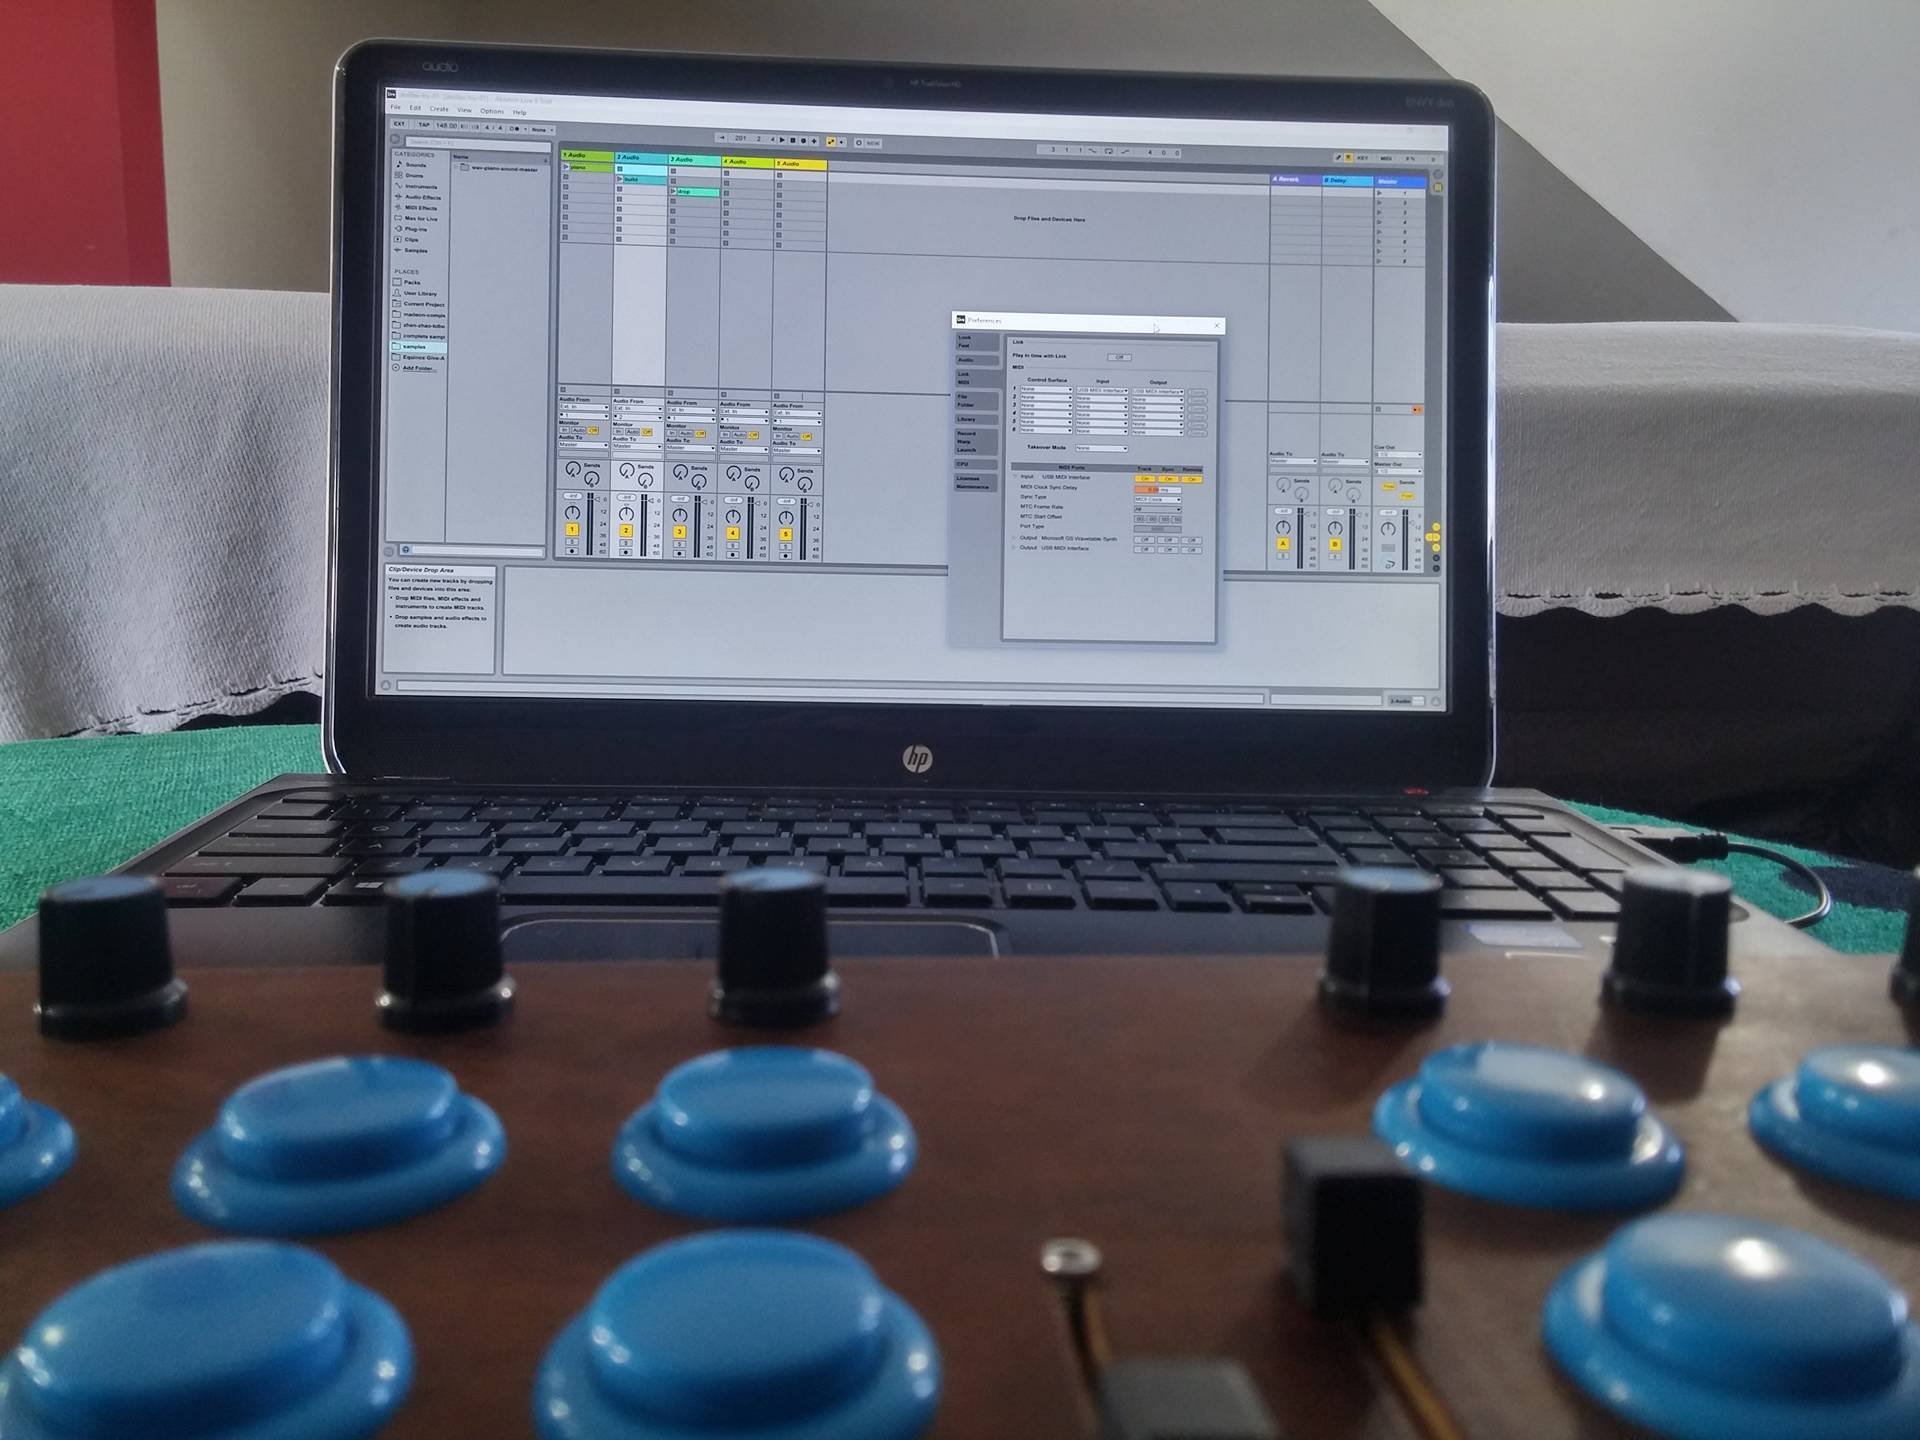
\includegraphics[scale=0.08]{Imagens/ableton2.jpg}
                            	\caption[Dalle pad com conexão MIDI]{Dalle pad com conexão MIDI}
                            	\label{fig:linear-pot}
                            \end{subfigure}
                        \end{figure}


            \end{frame}

            \begin{frame}\frametitle{Conexão MIDI com programa terceirizado}

                        \begin{figure}[H]
                        	\centering
                        	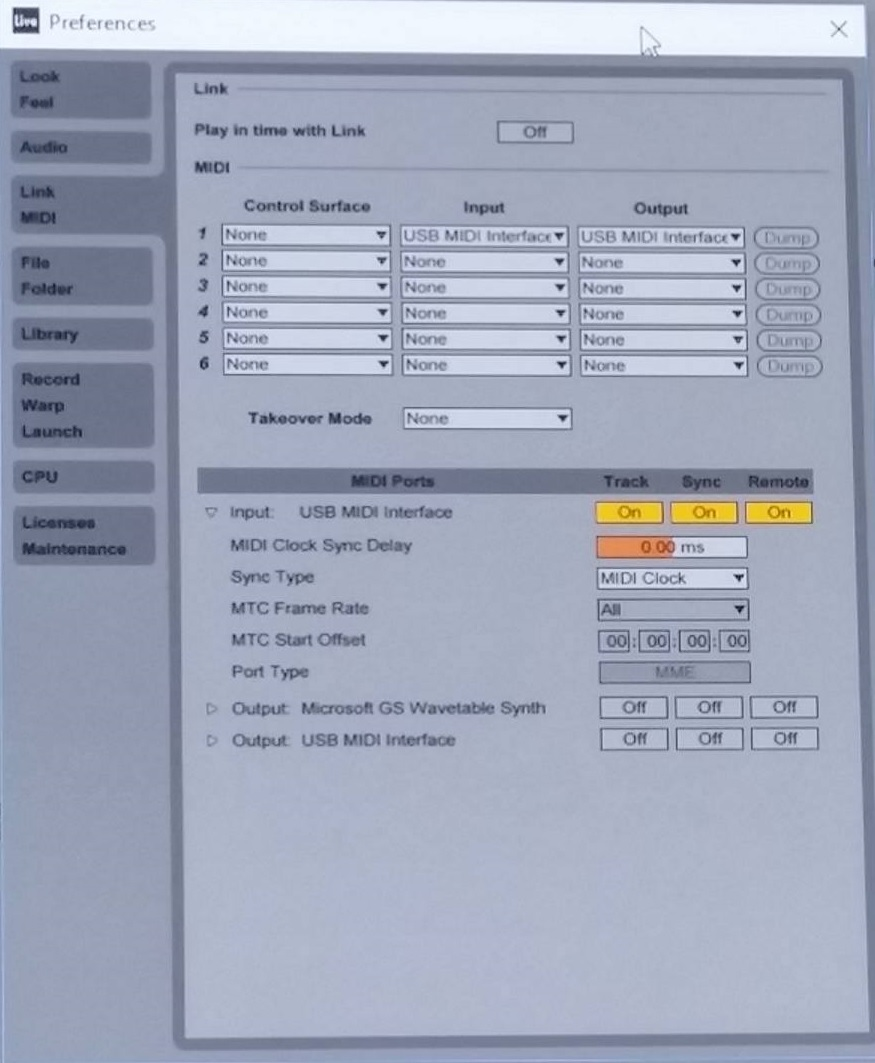
\includegraphics[scale=0.23]{Imagens/ableton3.jpg}
                        	\caption[Dalle Pad conectado com Ableton (Ampliado)]{Dalle Pad conectado com Ableton (Ampliado)}
                        	\label{fig:visao-geral}
                        \end{figure}

            \end{frame}

        \section{Estrutura}

            \begin{frame}\frametitle{Estrutura}

                \begin{itemize}
                  \item Projeto Mecânico - \textit{SOLIDWORKS}\copyright
                    \begin{itemize}
                      \item Versão em Plástico - Impressora 3D;
                      \item Versão em Madeira - Final.
                    \end{itemize}
                \end{itemize}

                \begin{figure}[H]
                    \centering
                    \begin{subfigure}[b]{.45\textwidth}
                        \centering
                        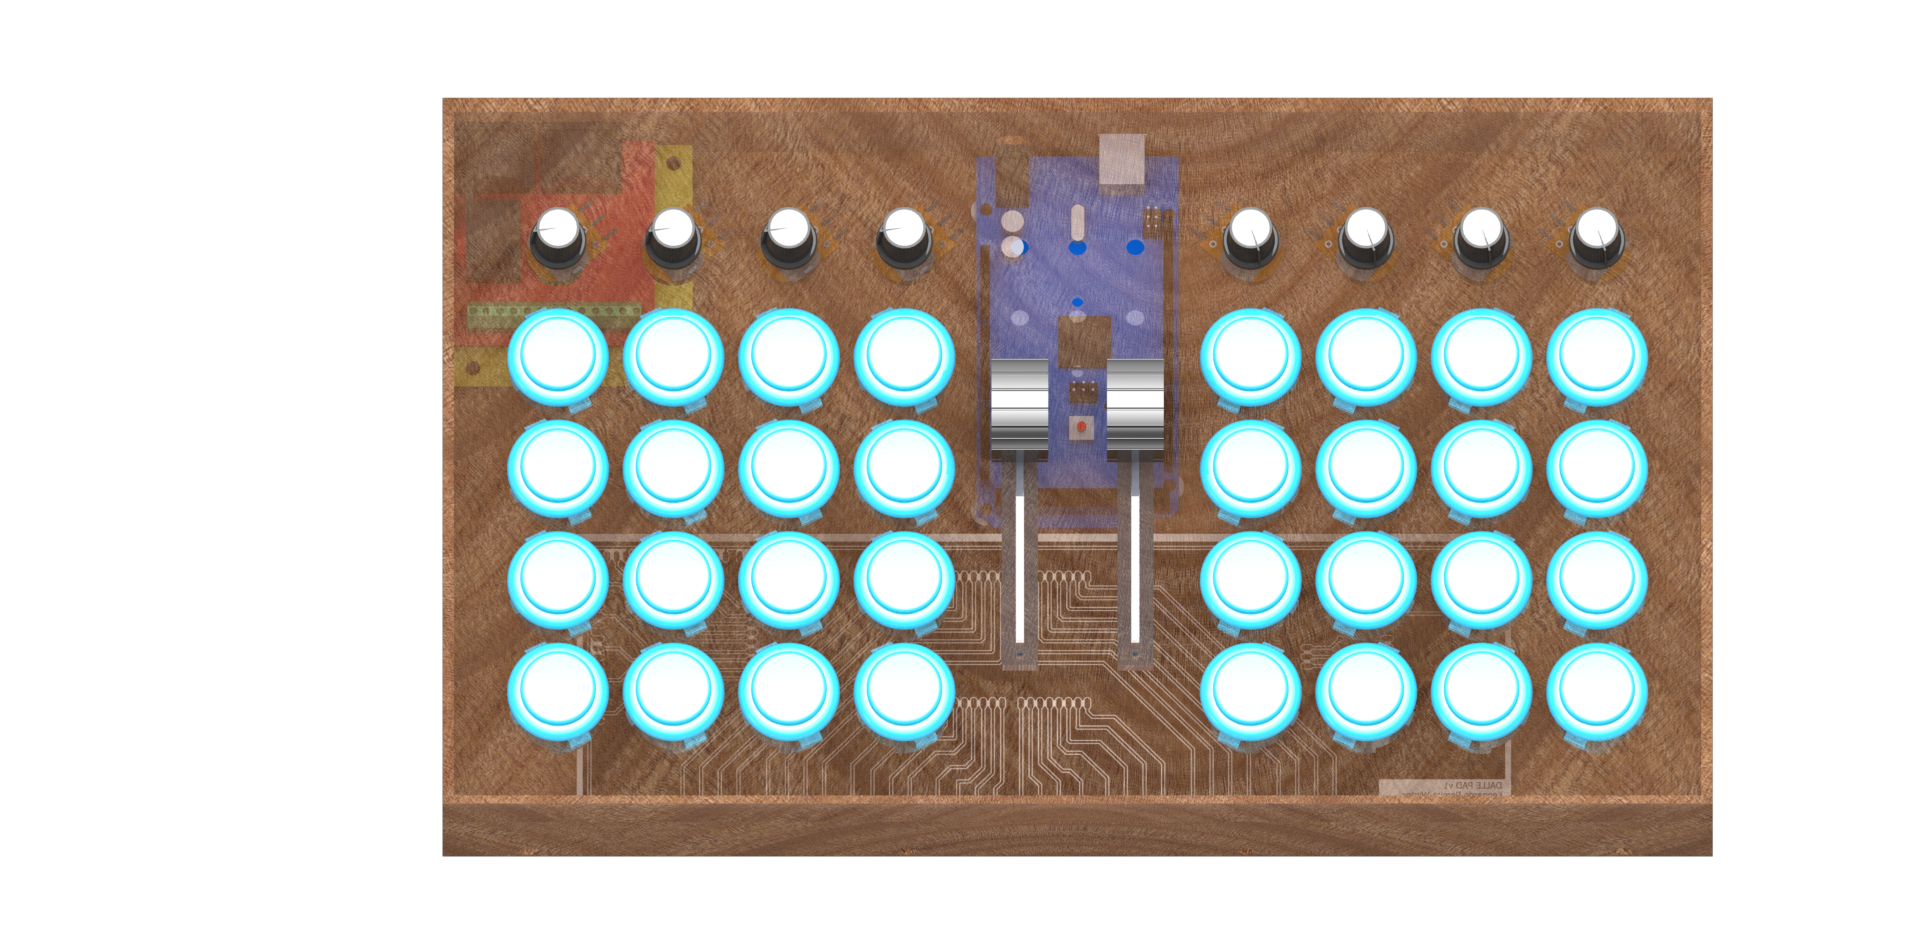
\includegraphics[scale=0.34]{Imagens/SW_Images/Involucro-de-Madeira/madeira10001.png}
                    	\caption[Visão Superior]{Visão Superior}
                        \label{fig:shield-midi}
                    \end{subfigure} %
                    \begin{subfigure}[b]{.45\textwidth}
                        \centering
                        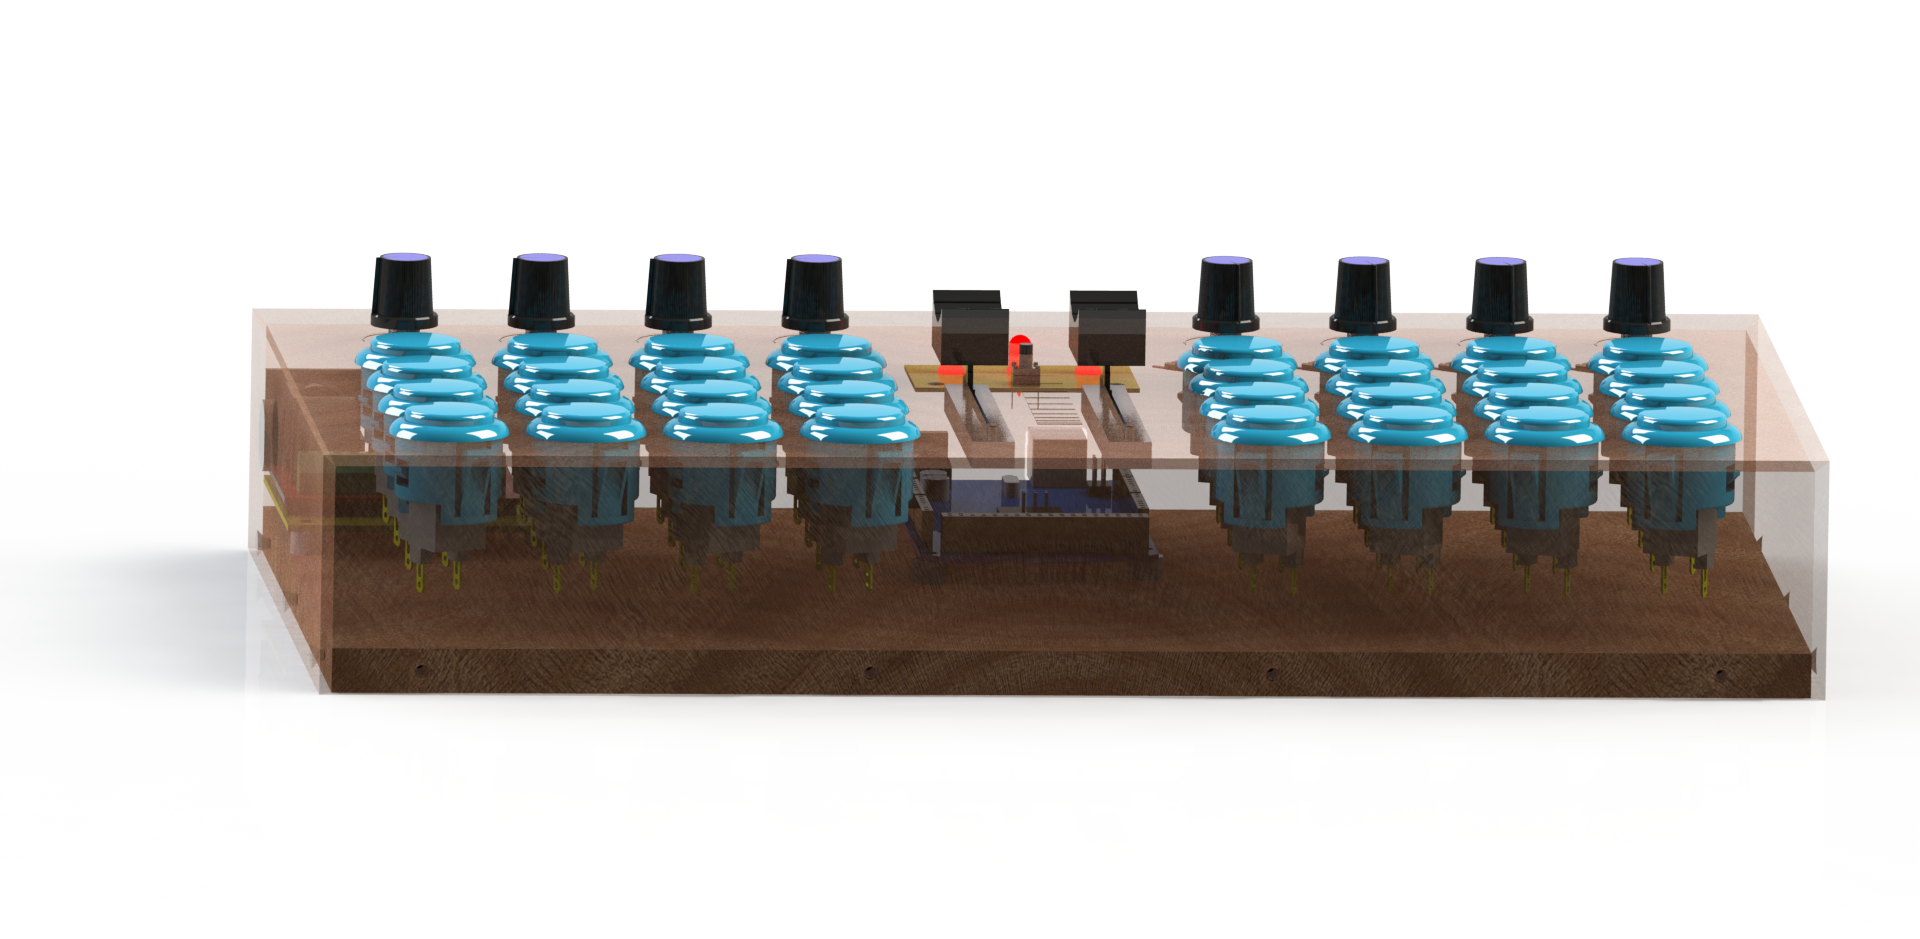
\includegraphics[scale=0.34]{Imagens/SW_Images/Involucro-de-Madeira/madeira5.png}
                    	\caption[Visão Ortogonal]{Visão Ortogonal}
                    	\label{fig:linear-pot}
                    \end{subfigure}

                    %\caption{Invólucro - Madeira}
                    \label{fig:madeiratriplex}
                \end{figure}

            \end{frame}

            \begin{frame}\frametitle{Estrutura}

                \begin{itemize}
                  \item Terceirização e Montagem:
                        \begin{figure}[H]
                            \centering
                            \begin{subfigure}[b]{.45\textwidth}
                                \centering
                                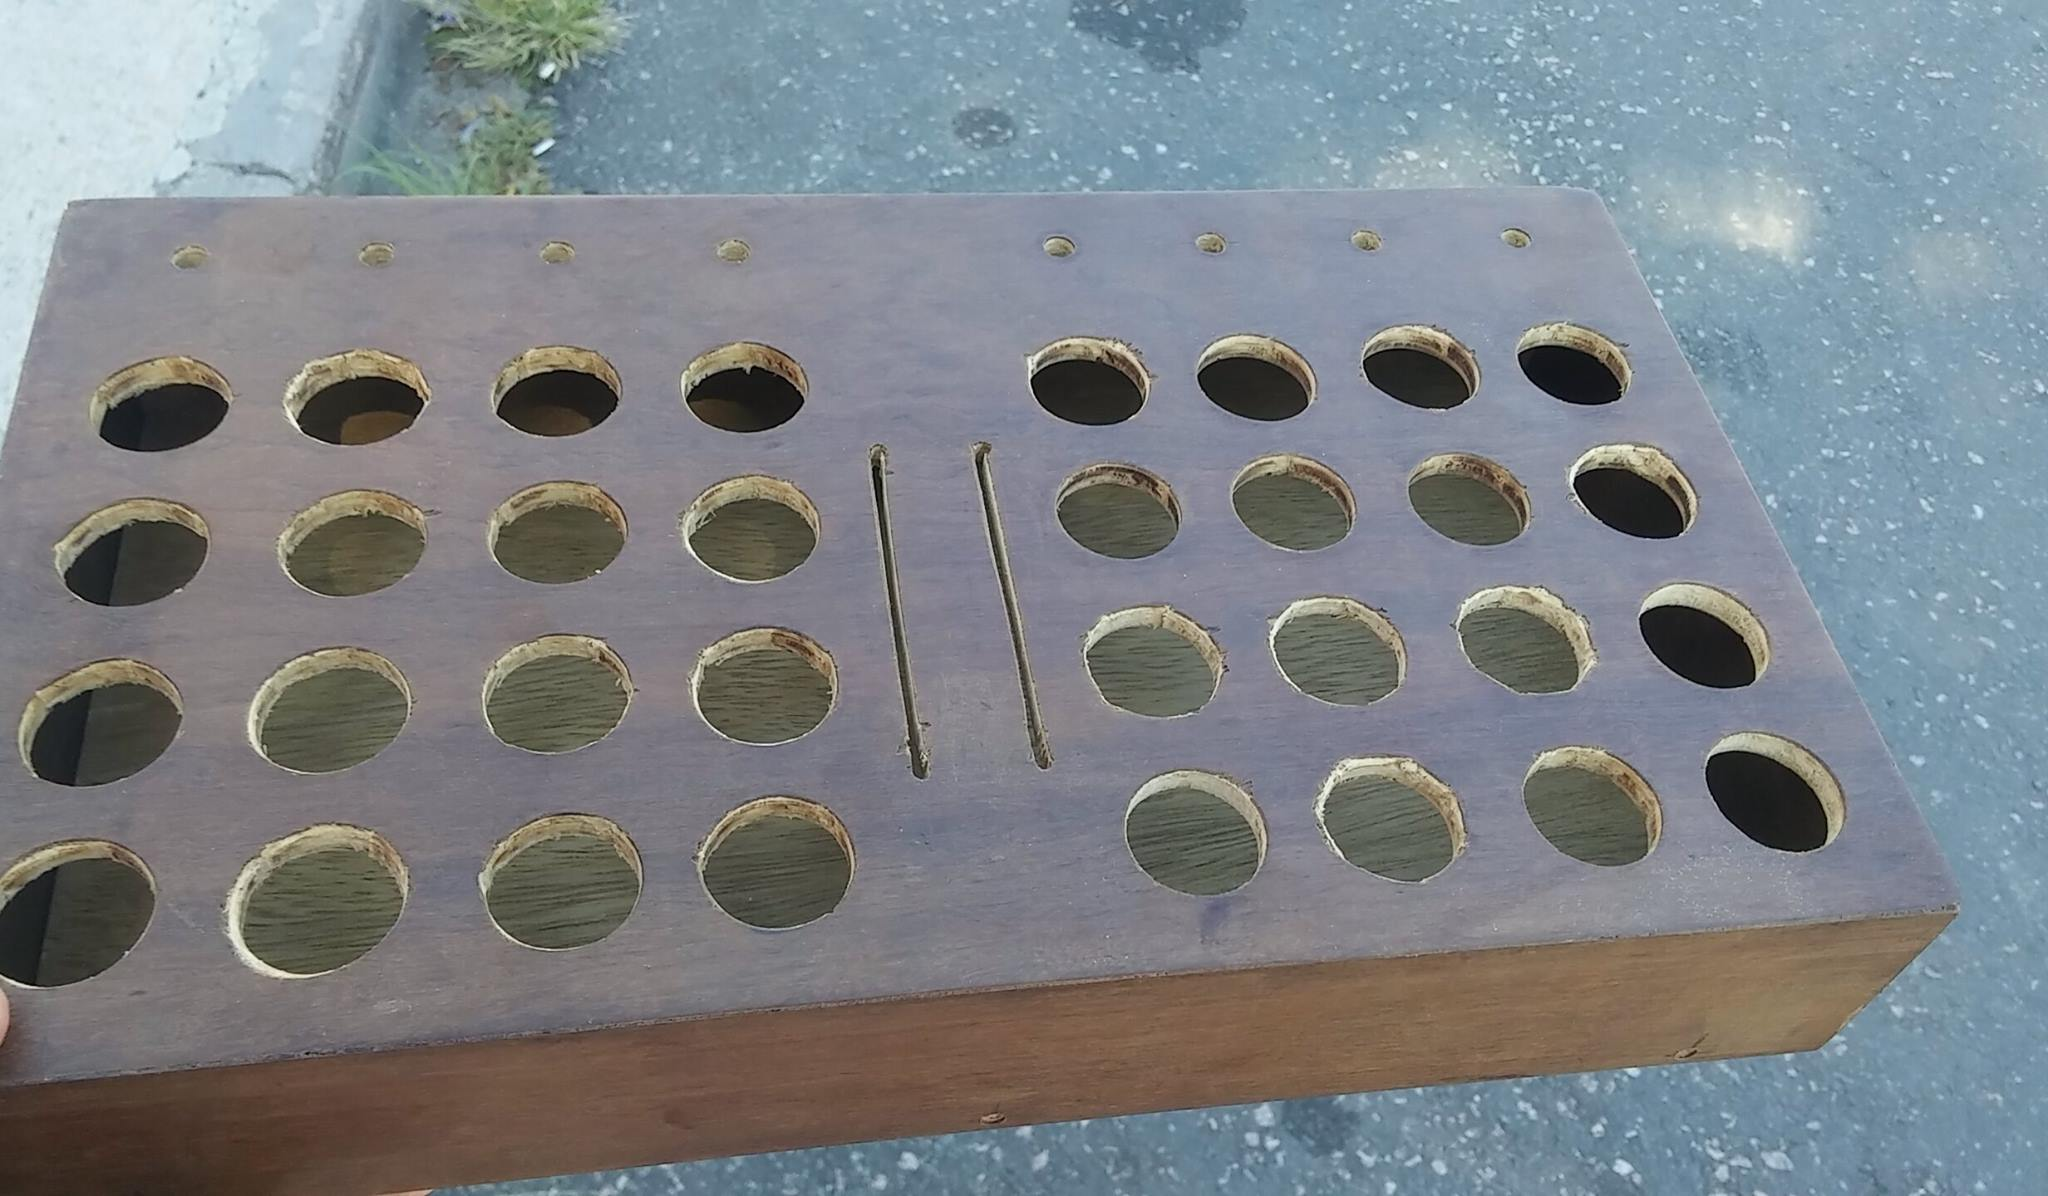
\includegraphics[scale=0.05]{Imagens/x002.jpg}
                            	\caption[Visão Superior]{Visão Superior}
                            	\label{fig:x002}
                            \end{subfigure} %
                            \begin{subfigure}[b]{.45\textwidth}
                                \centering
                            	\includegraphics[scale=0.073]{Imagens/backview.png}
                            	\caption[Visão Inferior]{Visão inferior}
                            	\label{fig:backview}
                            \end{subfigure}

                            %\caption{Invólucro}
                            \label{fig:madeiratriplex}
                        \end{figure}

                  \item Produto Final:
                        \begin{figure}[H]
                        	\centering
                        	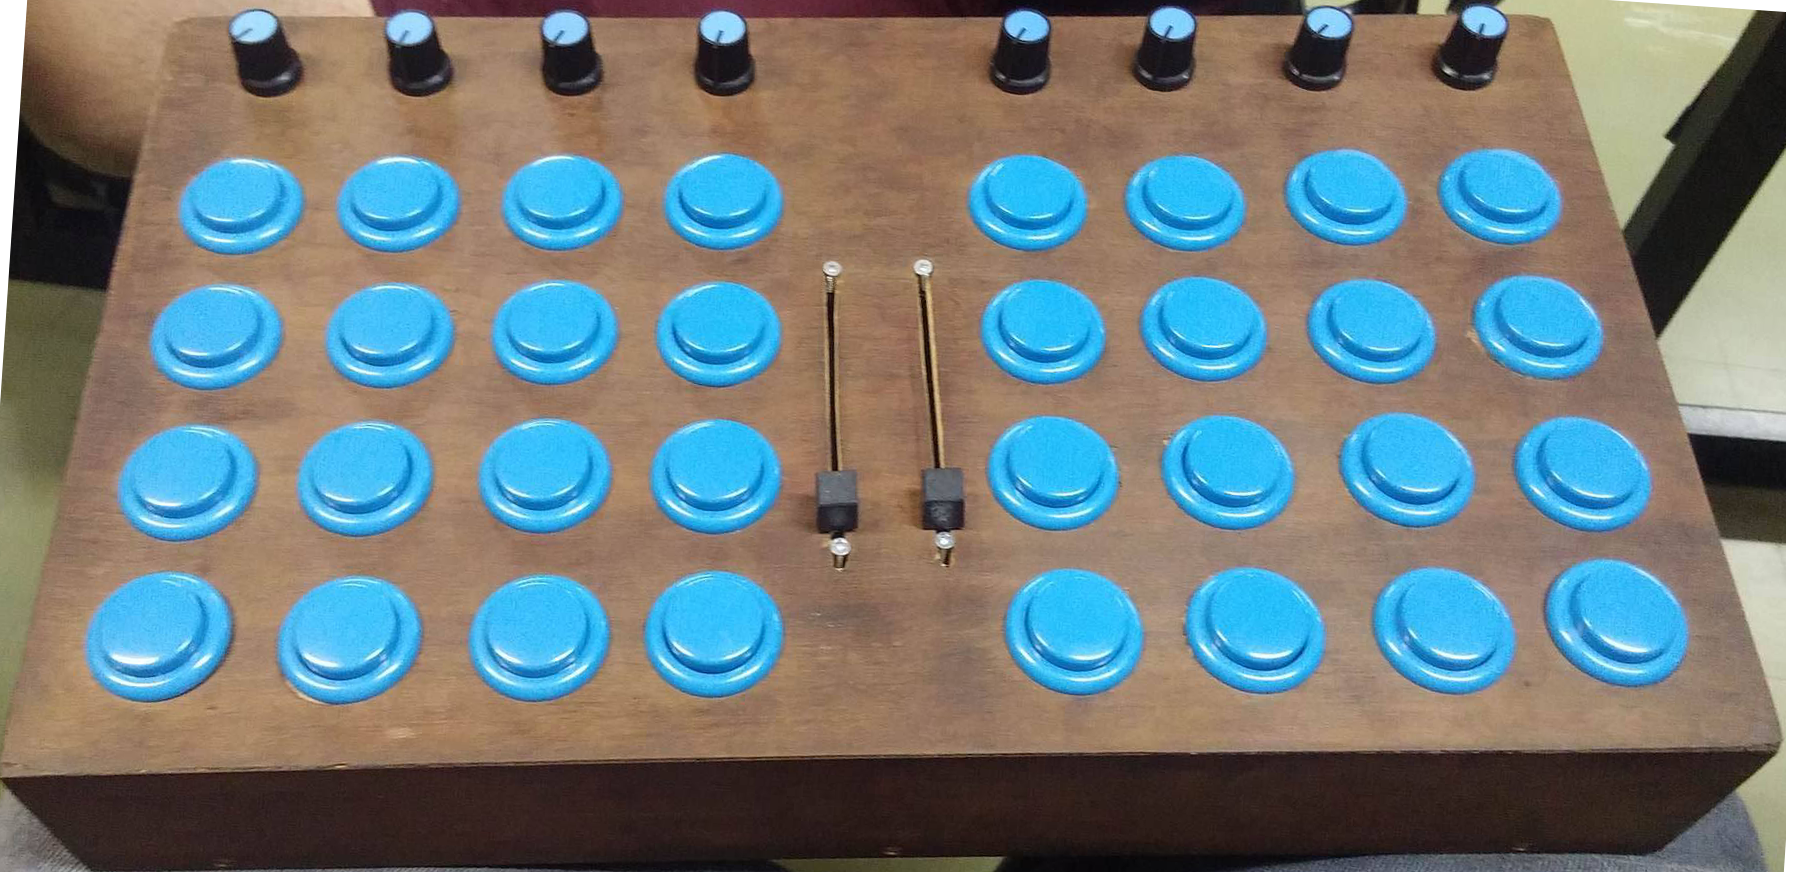
\includegraphics[scale=0.1]{Imagens/x02.png}
                        	\caption[Visão do produto final]{Visão do produto final}
                        	\label{fig:requisitos}
                        \end{figure}
                \end{itemize}

            \end{frame}

        \section{Sistema Embarcado e Estação Base}

            \subsection{Sistema Embarcado}

                \begin{frame}\frametitle{Diagrama de Blocos}

                    \begin{figure}[H]
                    	\centering
                    	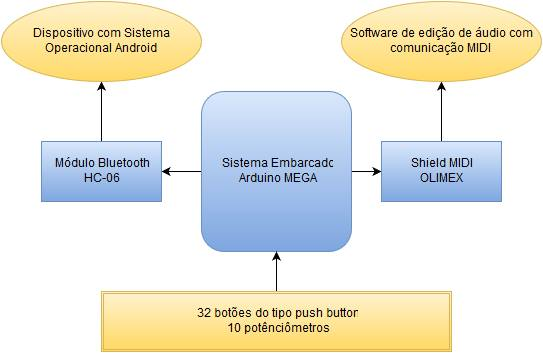
\includegraphics[scale=0.4]{Imagens/Zi04.jpg}
                    	\caption[Diagrama de Blocos]{Diagrama de Blocos}
                    	\label{fig:requisitos}
                    \end{figure}

                \end{frame}

                \begin{frame}\frametitle{Sistema Embarcado e Módulos}

                    \begin{figure}[H]
                        \centering
                        \begin{subfigure}[b]{.45\textwidth}
                            \centering
                            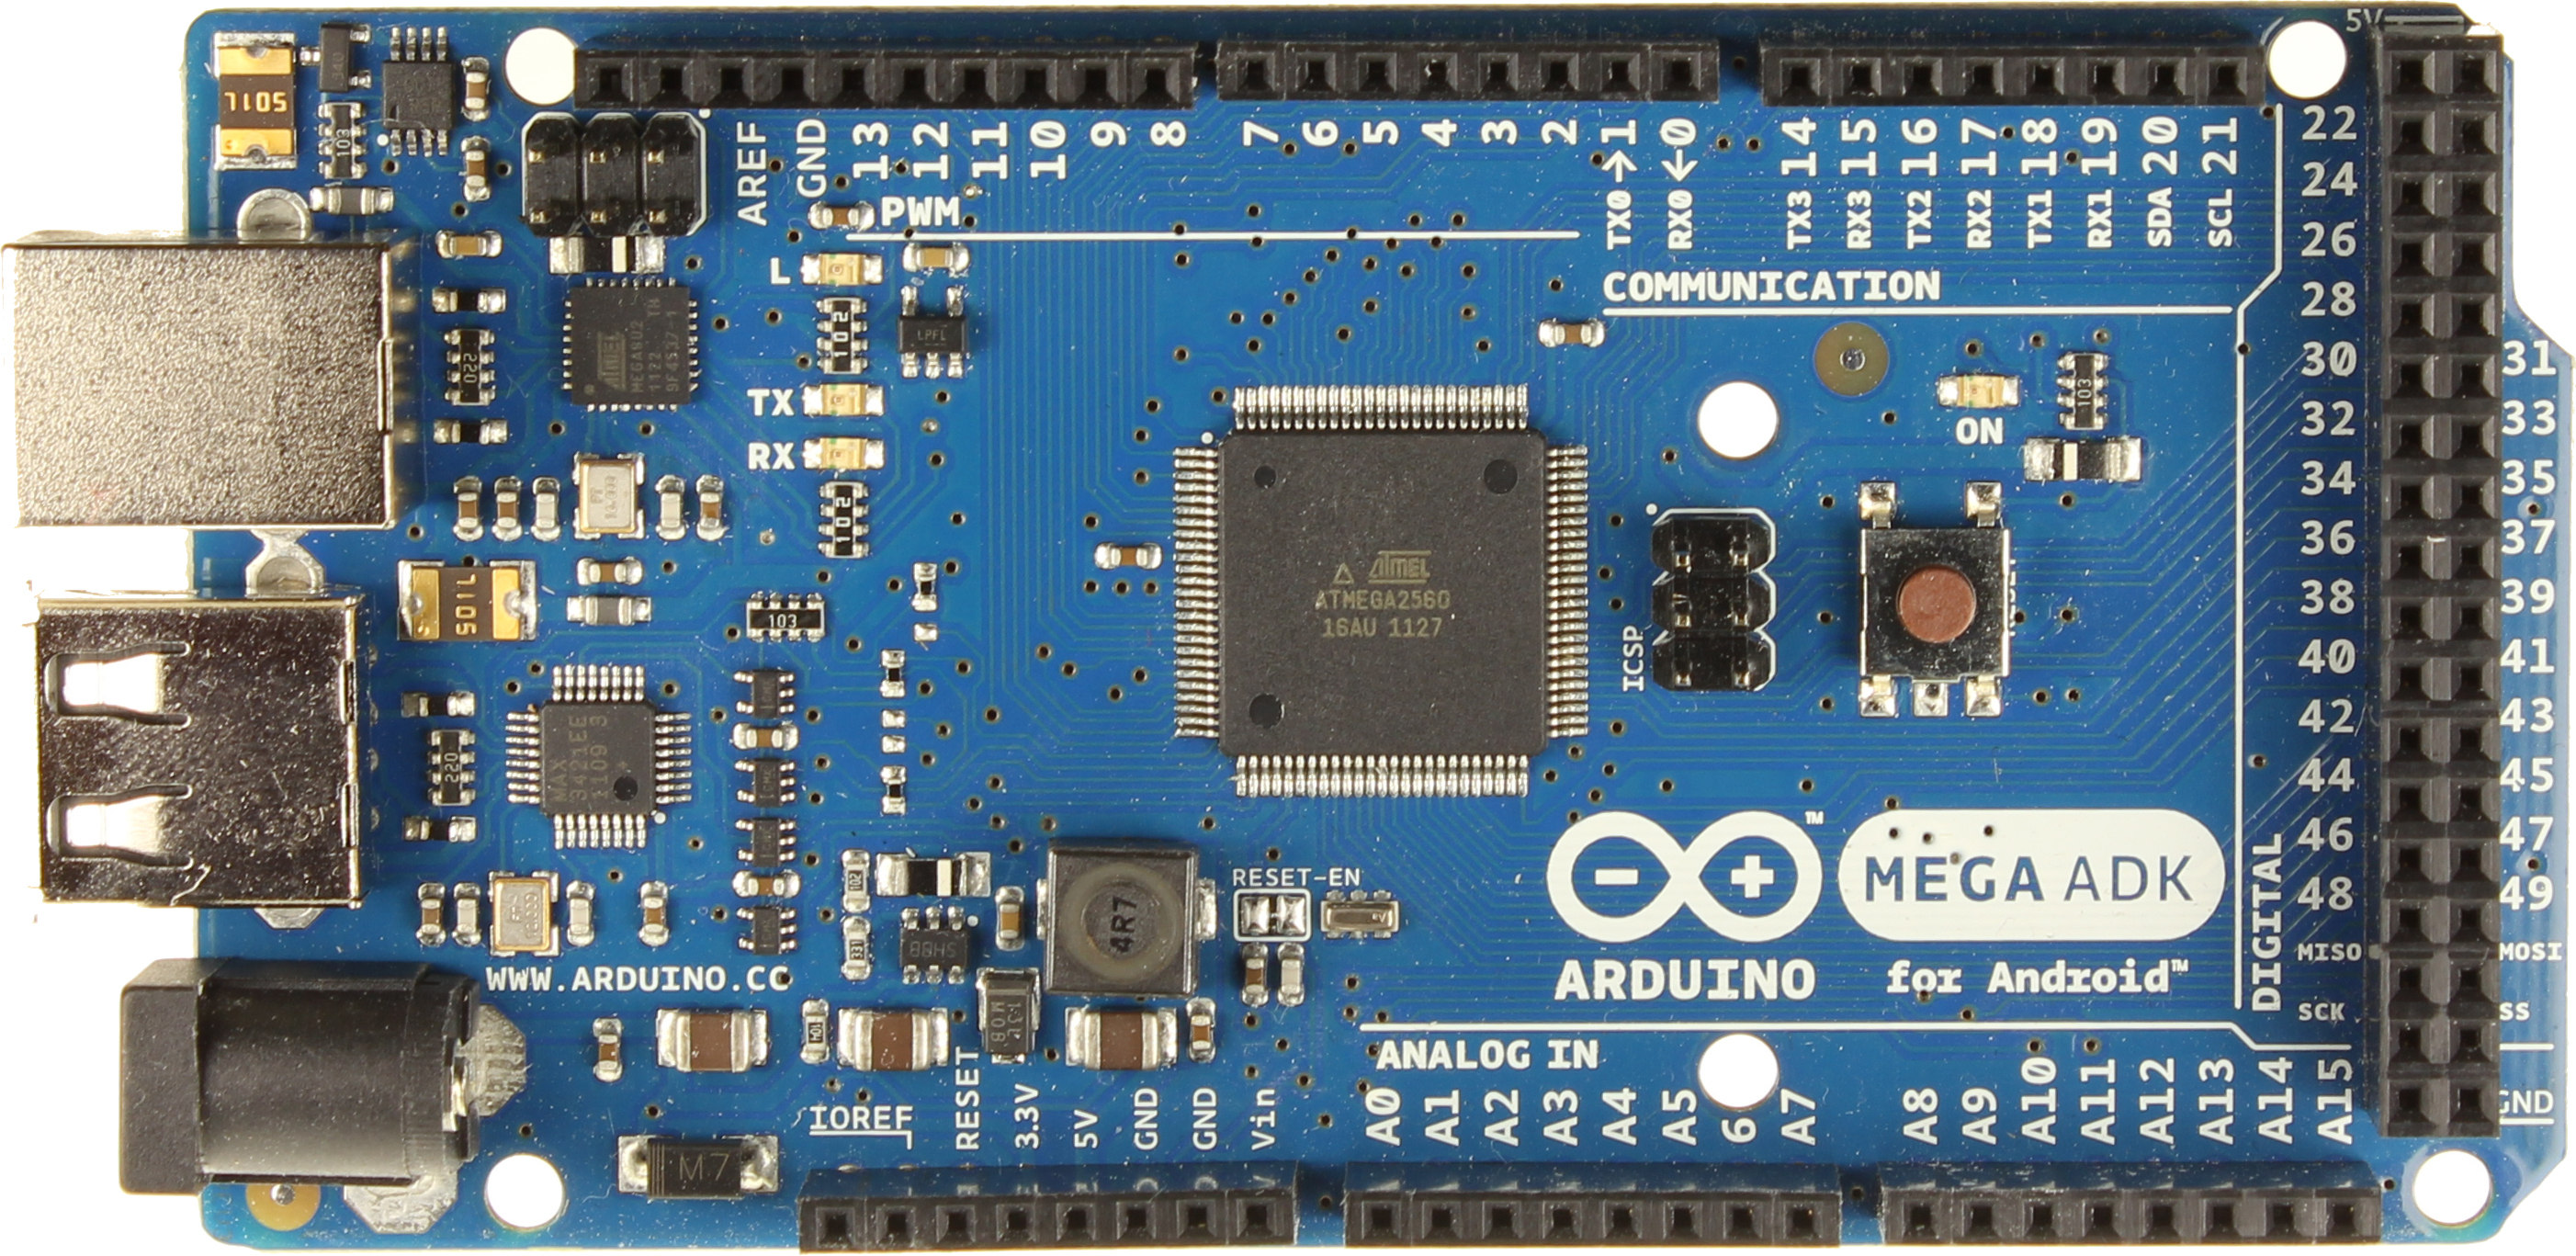
\includegraphics[scale=0.05]{Imagens/Zi05.jpg}
                        	\caption[Arduino MEGA2560]{Arduino MEGA2560}
                        	\label{fig:x002}
                        \end{subfigure} %
                        \begin{subfigure}[b]{.45\textwidth}
                            \centering
                        	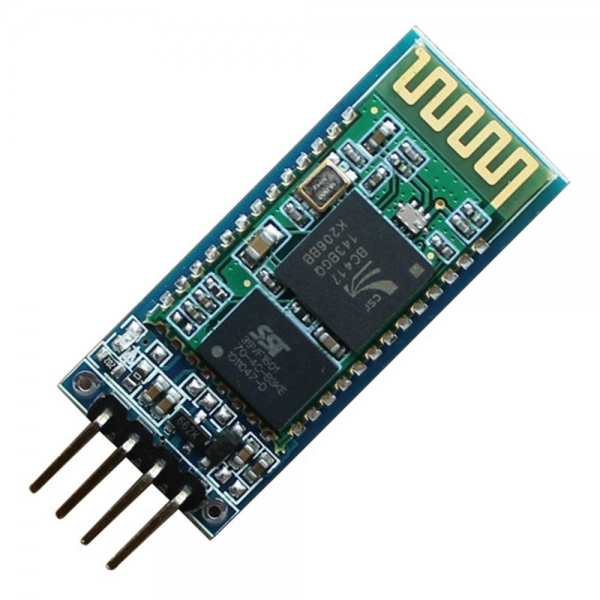
\includegraphics[scale=0.10]{Imagens/Zi06.jpg}
                        	\caption[Módulo \textit{Bluetooth} HC06]{Módulo \textit{Bluetooth} HC06}
                        	\label{fig:backview}
                        \end{subfigure}

                        \begin{subfigure}[b]{.45\textwidth}
                            \centering
                        	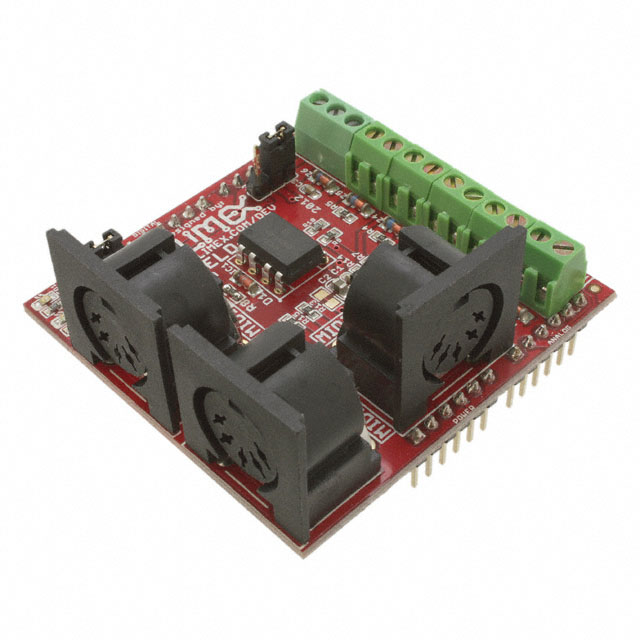
\includegraphics[scale=0.15]{Imagens/Zi07.jpg}
                        	\caption[\textit{Olimex Shield} MIDI]{\textit{Olimex Shield} MIDI}
                        	\label{fig:backview}
                        \end{subfigure}

                        %\caption{Invólucro}
                        \label{fig:madeiratriplex}
                    \end{figure}

                \end{frame}

                \begin{frame}\frametitle{Placa de Circuito}

                    \begin{figure}[H]
                    	\centering
                    	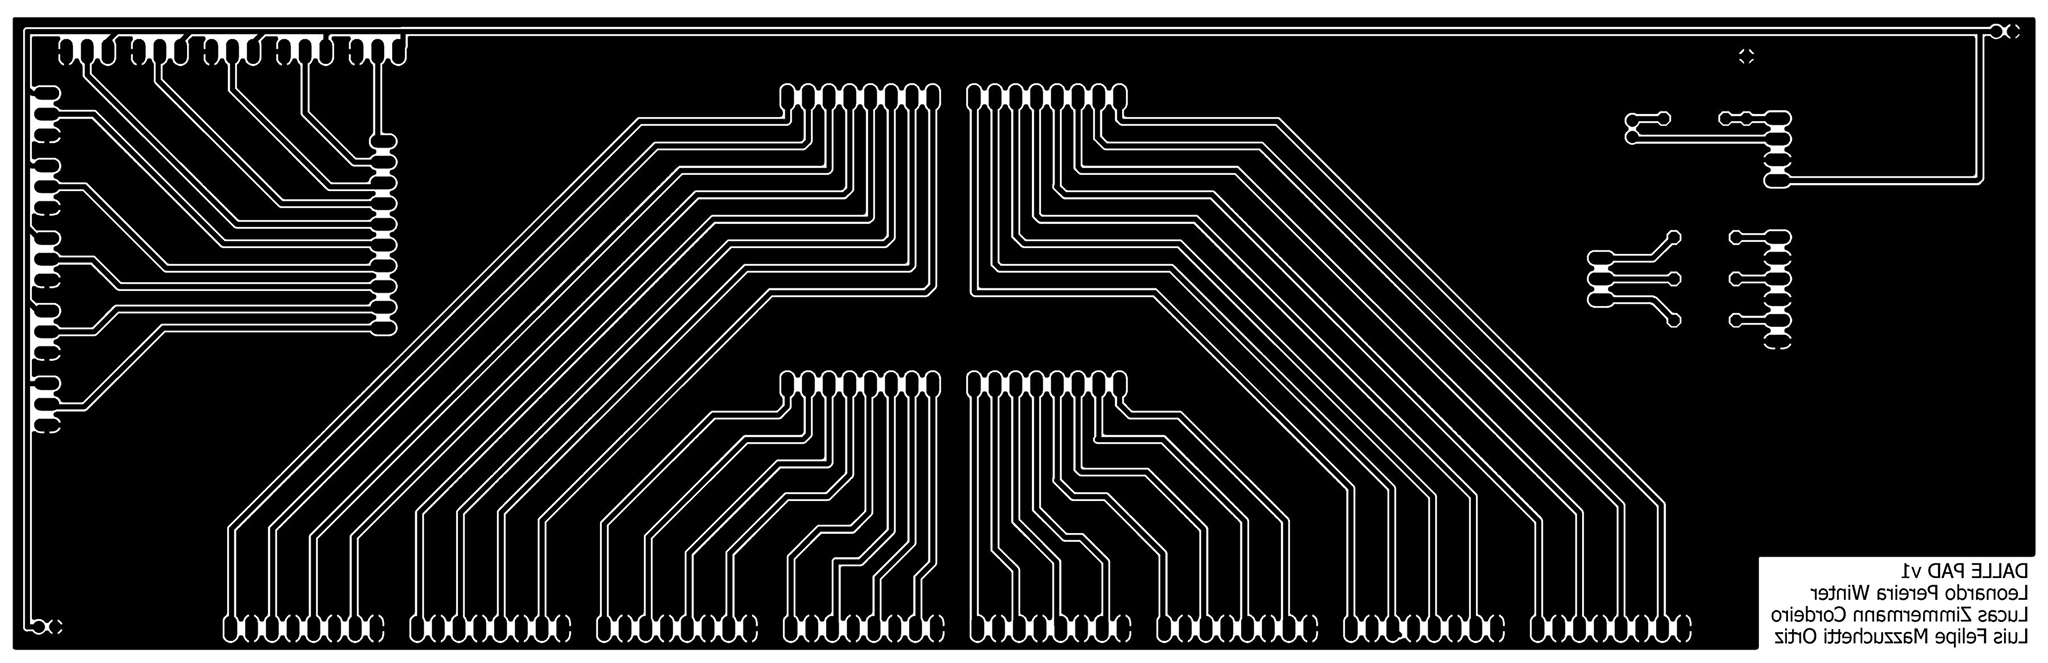
\includegraphics[scale=0.16]{Imagens/pcb.png}
                    	\caption[Layout da PCB desenvolvida pela equipe]{Layout da PCB desenvolvida pela equipe}
                    	\label{fig:requisitos}
                    \end{figure}

                \end{frame}

                \begin{frame}\frametitle{Placa Universal}

                    \begin{figure}[H]
                    	\centering
                    	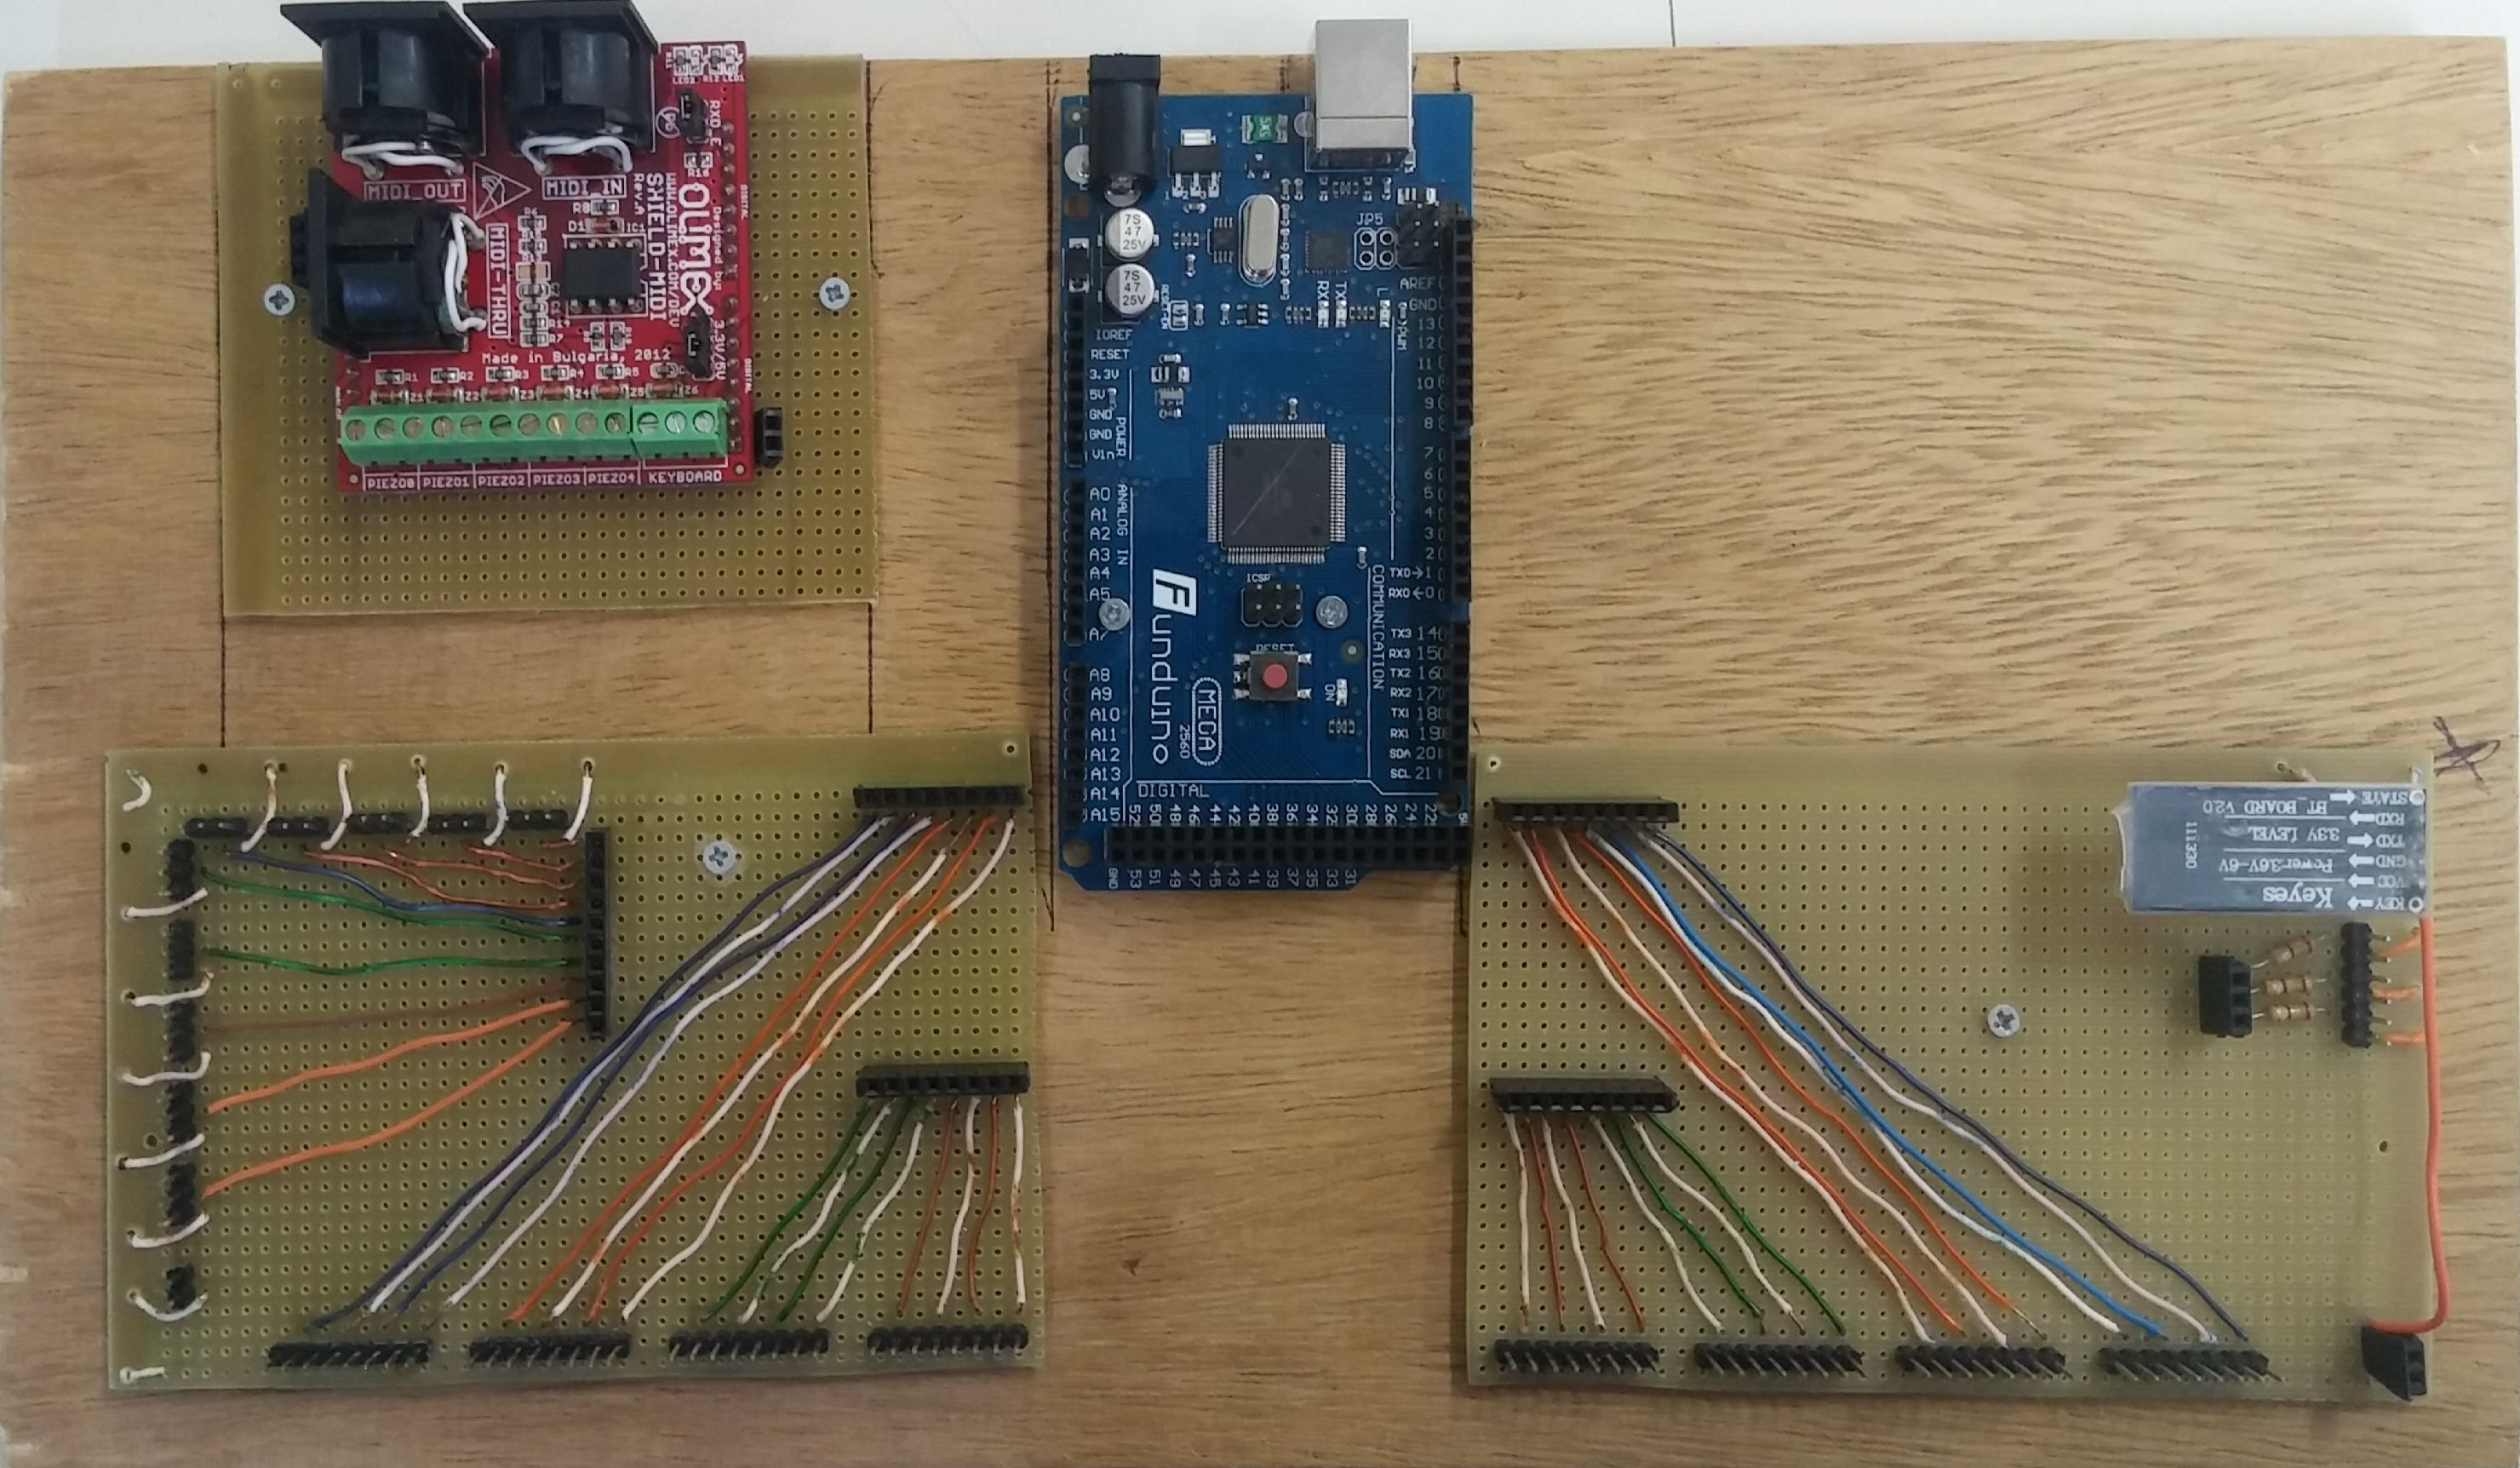
\includegraphics[scale=0.10]{Imagens/Zi01.jpg}
                    	\caption[Placa universal e módulos]{Placa universal e módulos}
                    	\label{fig:requisitos}
                    \end{figure}

                \end{frame}

                \begin{frame}\frametitle{Cabos}

                    \begin{figure}[H]
                        \centering
                        \begin{subfigure}[b]{.45\textwidth}
                            \centering
                            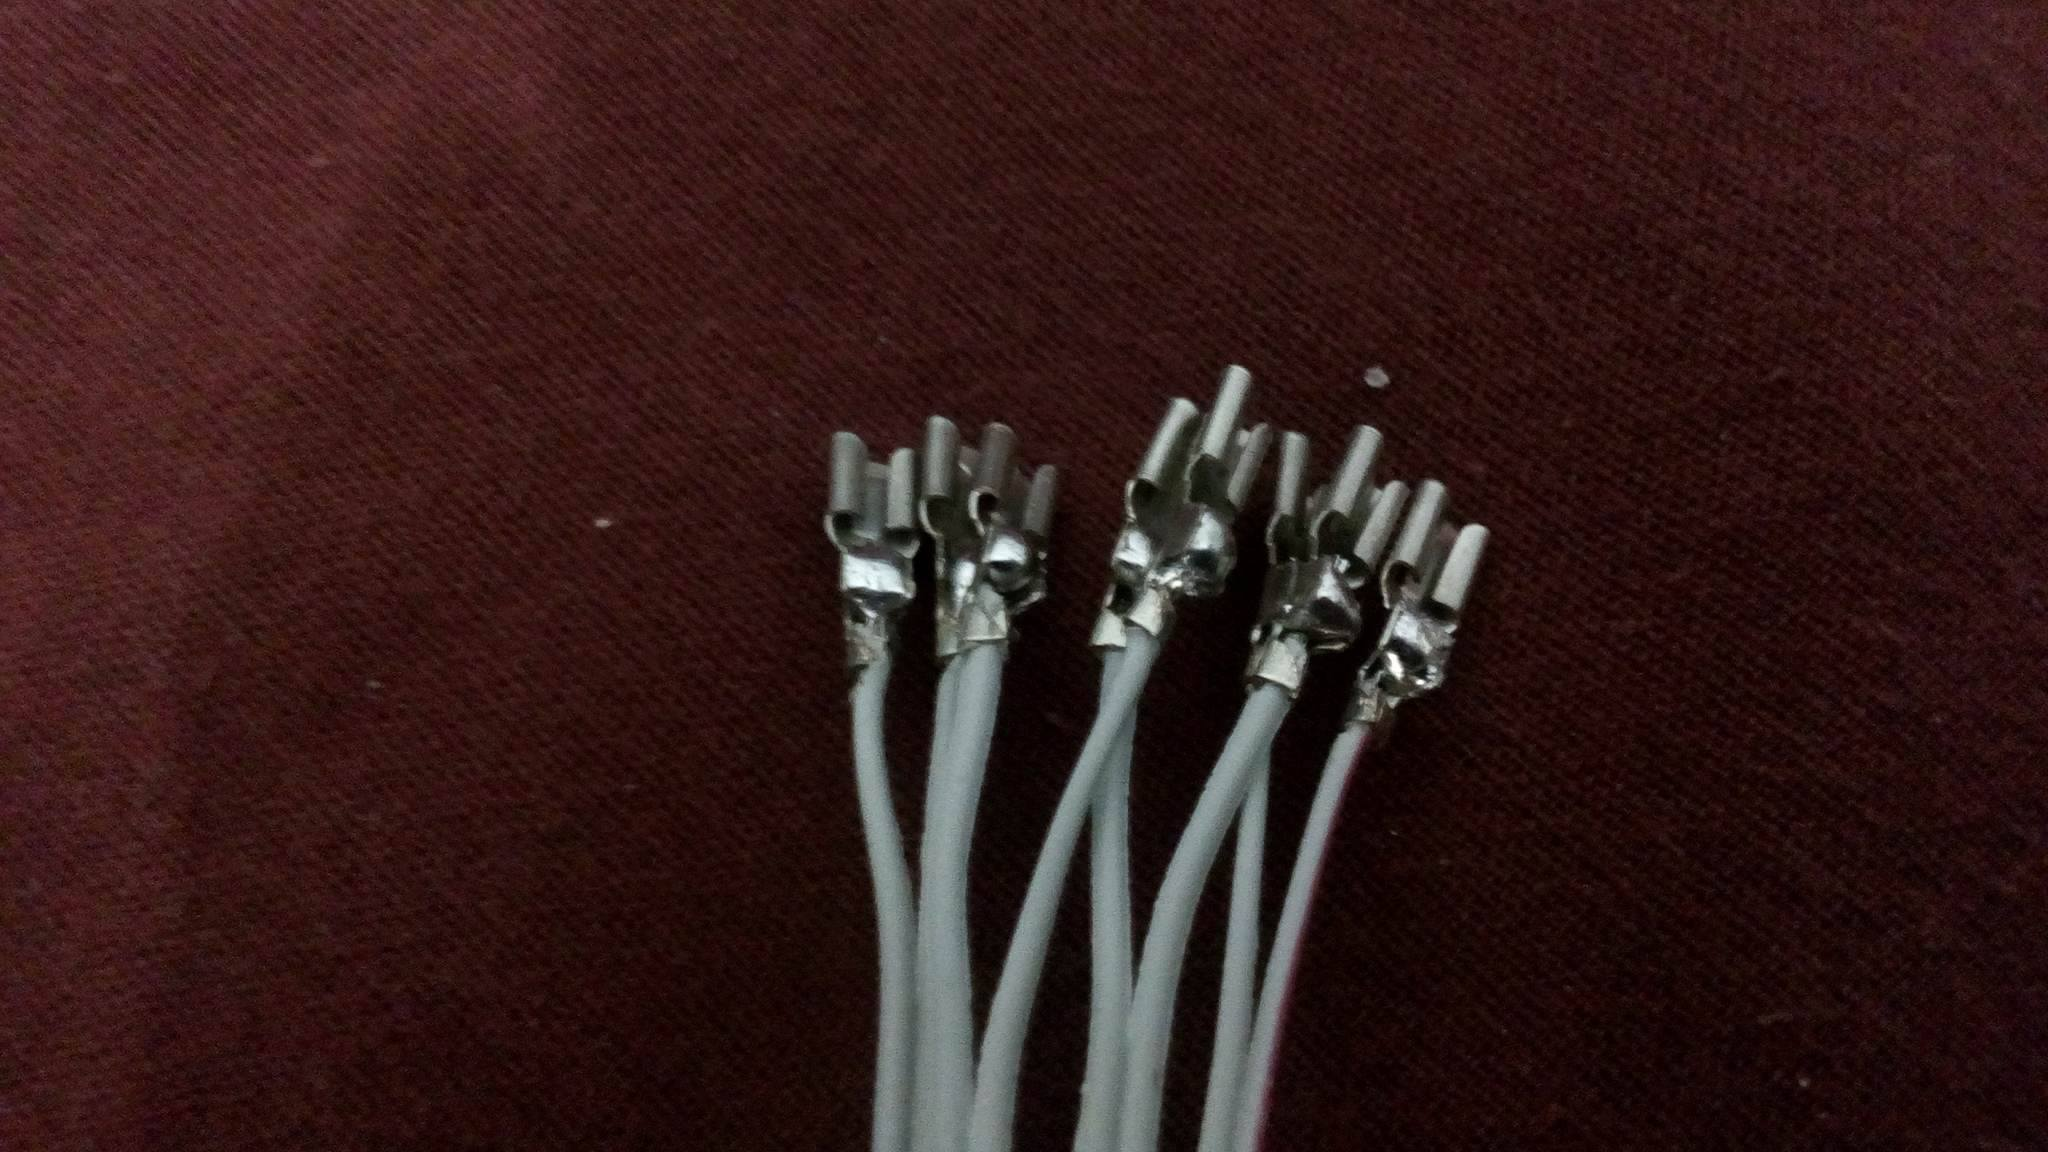
\includegraphics[scale=0.08]{Imagens/Zi02.jpg}
                        	\caption[Conectores \textit{Faston}]{Conectores \textit{Faston}}
                        	\label{fig:x002}
                        \end{subfigure} %
                        \begin{subfigure}[b]{.45\textwidth}
                            \centering
                        	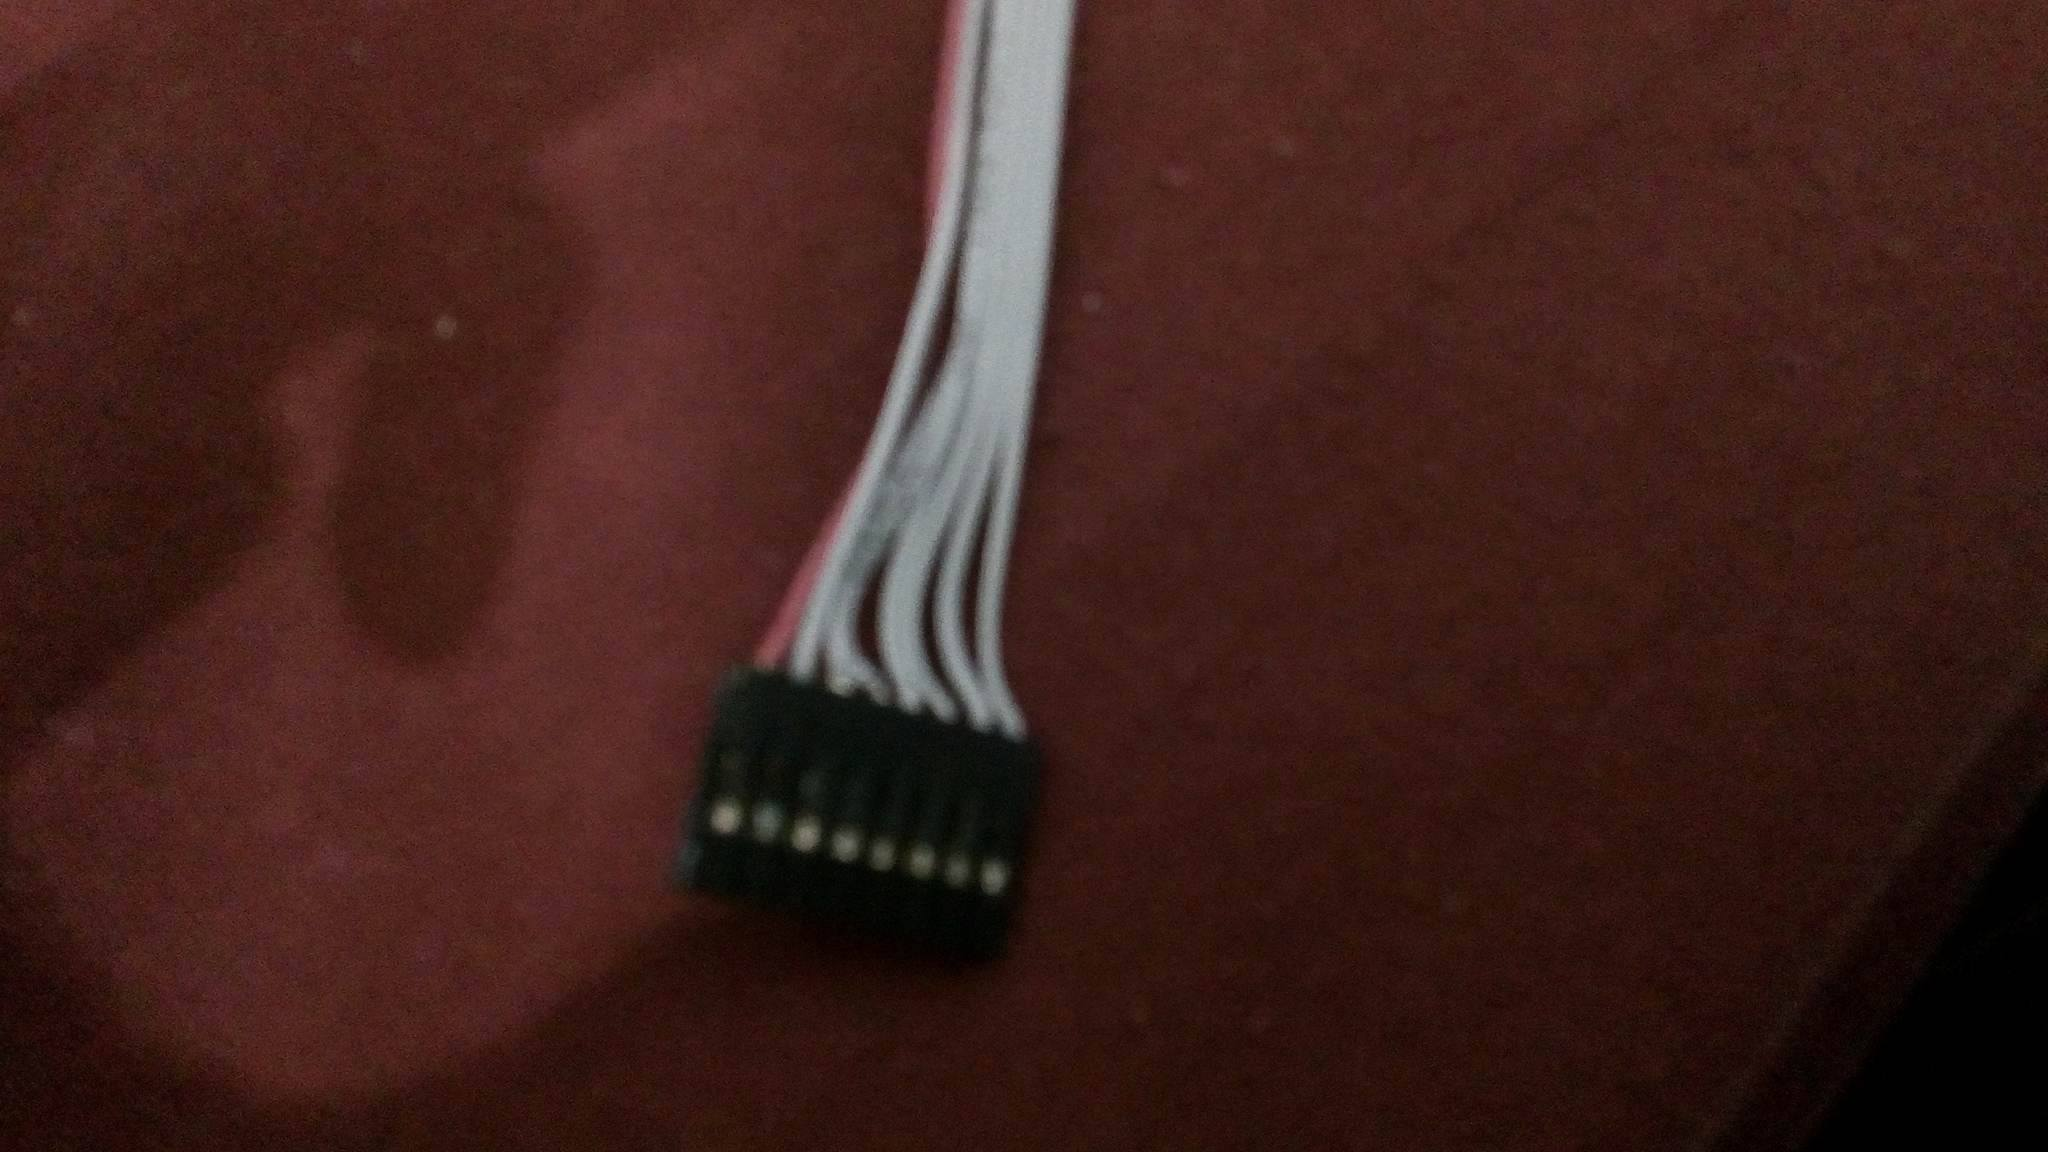
\includegraphics[scale=0.08]{Imagens/Zi03.jpg}
                        	\caption[Barra de pinos]{Barra de pinos}
                        	\label{fig:backview}
                        \end{subfigure}

                        %\caption{Invólucro}
                        \label{fig:madeiratriplex}
                    \end{figure}

                \end{frame}

            \subsection{Estação Base}

                \begin{frame}\frametitle{Estação Base}

                     \begin{itemize}
                      \item Aplicativo para Android:
                        \begin{itemize}
                          \item Reprodução de áudio;
                          \item Mudança de efeitos;
                        \end{itemize}
                    \end{itemize}

                    \begin{figure}[H]
                        \centering
                        \begin{subfigure}[b]{.45\textwidth}
                            \centering
                            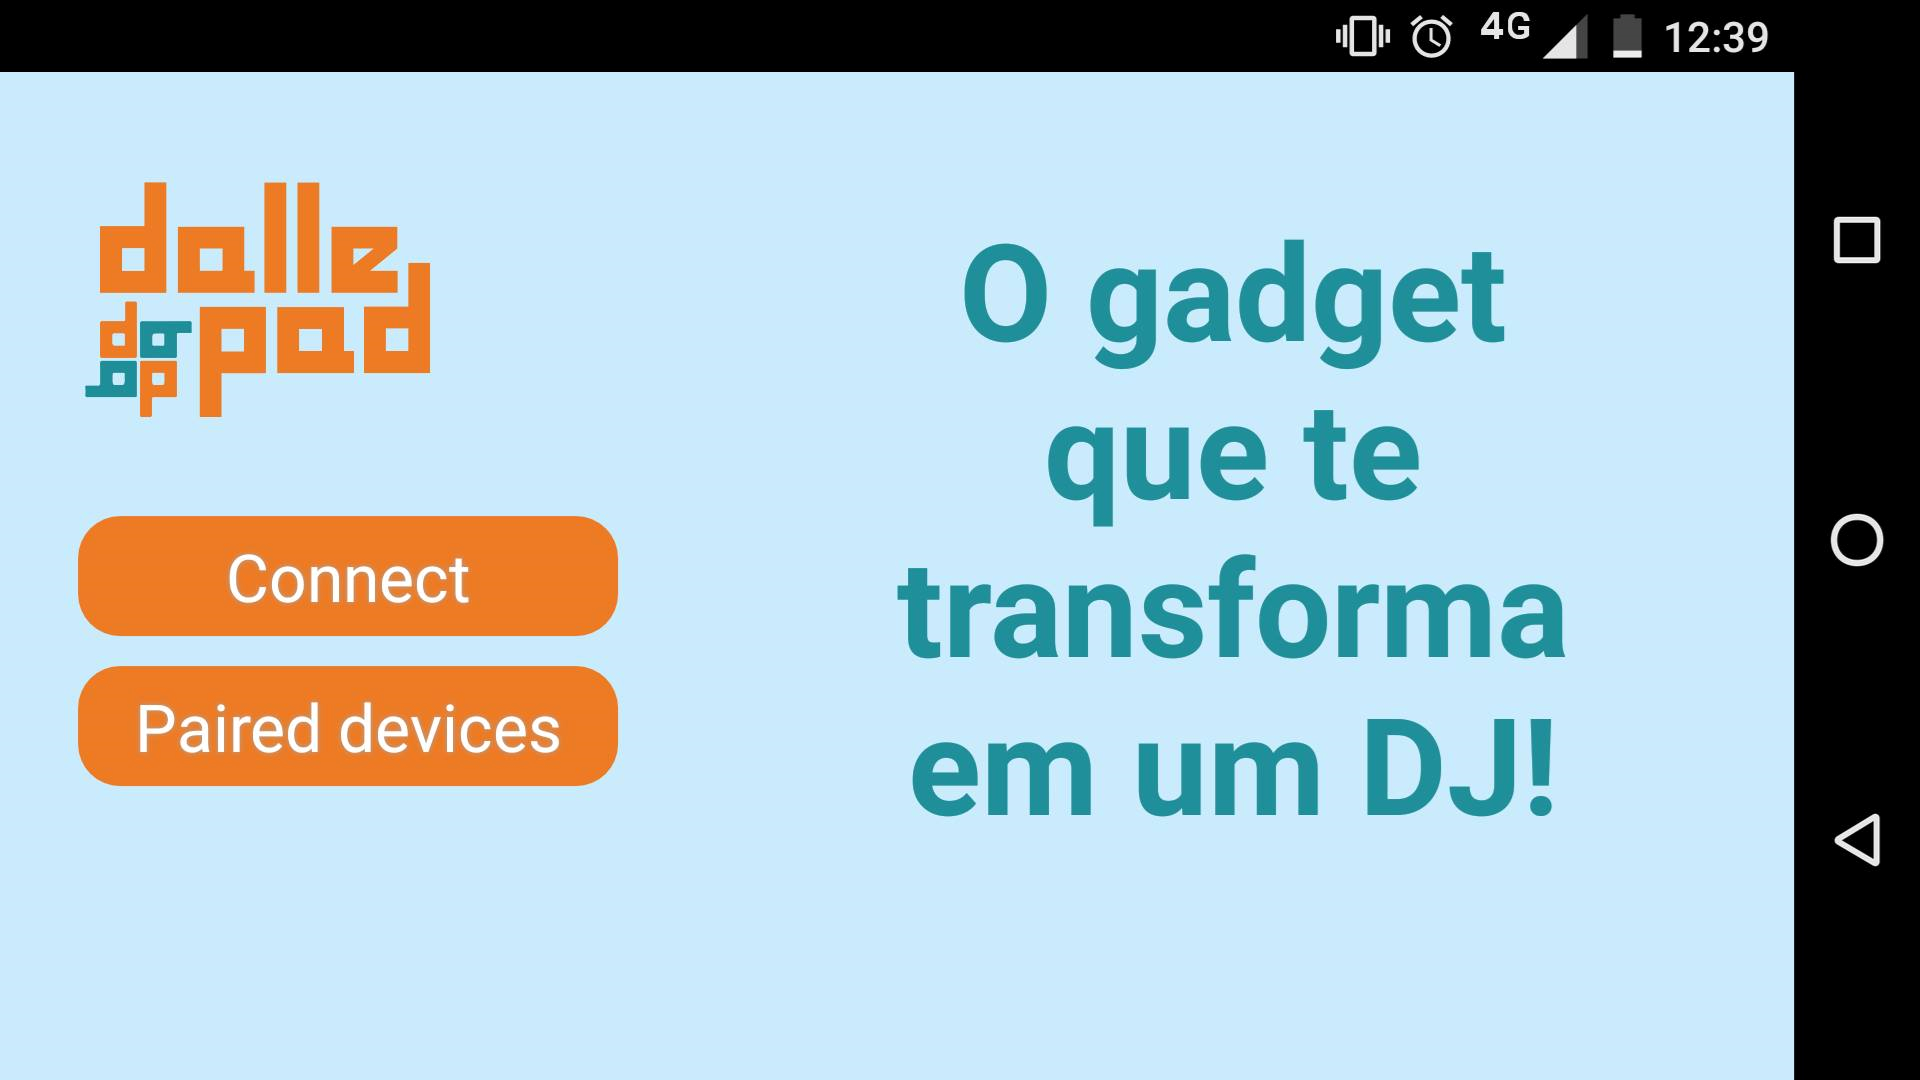
\includegraphics[scale=0.13]{Imagens/mainview.png}
                        	\caption[Tela \textit{MainView}]{Tela \textit{MainView}}
                            \label{fig:43}
                        \end{subfigure} %
                        \begin{subfigure}[b]{.45\textwidth}
                            \centering
                            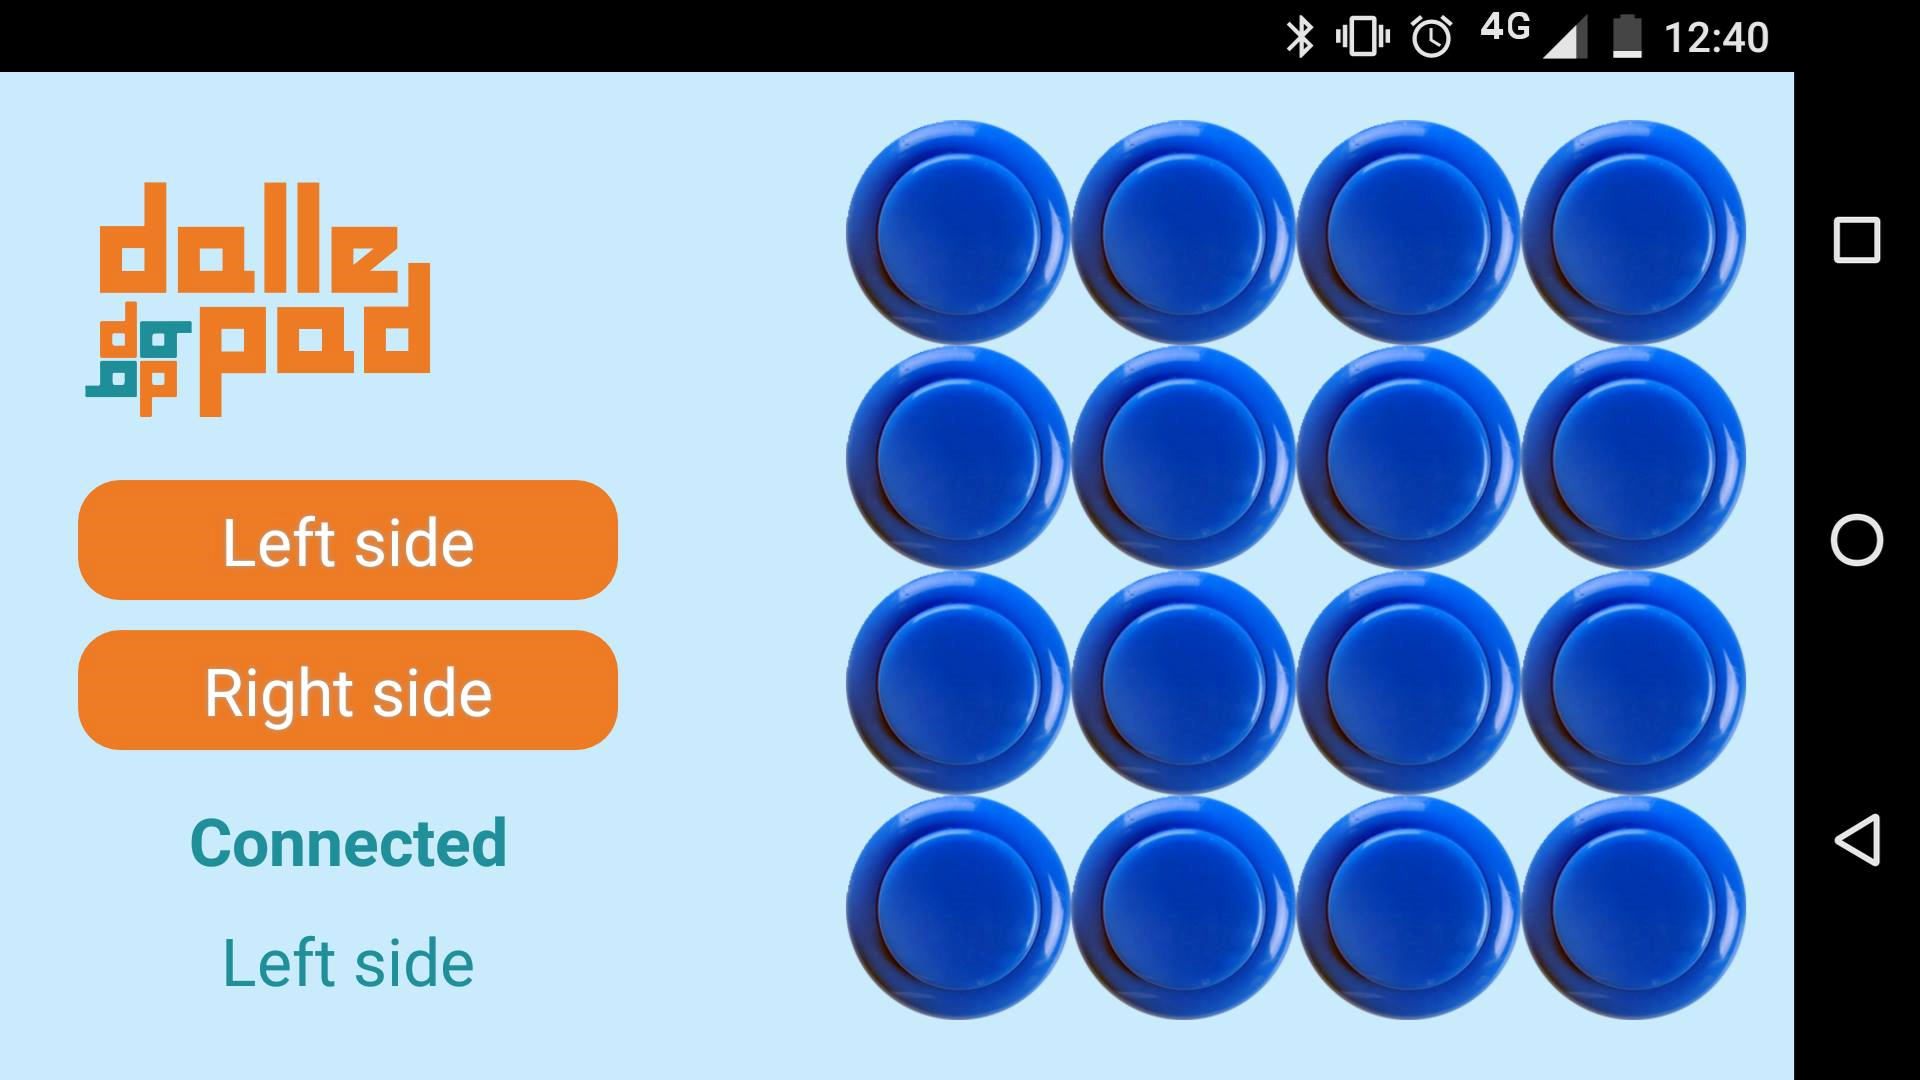
\includegraphics[scale=0.13]{Imagens/connectedview.png}
                        	\caption[Tela \textit{ConnectedView}]{Tela \textit{ConnectedView}}
                        	\label{fig:44}
                        \end{subfigure}

                        \label{fig:madeiratriplex}
                    \end{figure}

                \end{frame}

        \section{Algoritmos}

            \begin{frame}\frametitle{Algoritmos - Android}

                     \begin{itemize}
                      \item Aplicativo Android:
                        \begin{itemize}
                          \item Modelo MVC (\textit{Model-view-controller})
                          \item Classe Java \textit{BluetoothAdapter} e \textit{BluetoothSocket}
                          \item Classe Java \textit{SoundPool}
                        \end{itemize}
                    \end{itemize}

                    \begin{figure}[H]
                        \centering
                        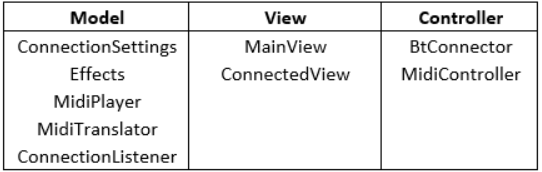
\includegraphics[scale=0.6]{Imagens/mvc.png}
                        \caption[Divisão das classes no modelo MVC]{Divisão das classes no modelo MVC}
                    \end{figure}

            \end{frame}

            \begin{frame}\frametitle{Algoritmos - Arduino}

                    \begin{itemize}
                        \item Arduino:
                    \end{itemize}

                    \begin{figure}[H]
                        \centering
                        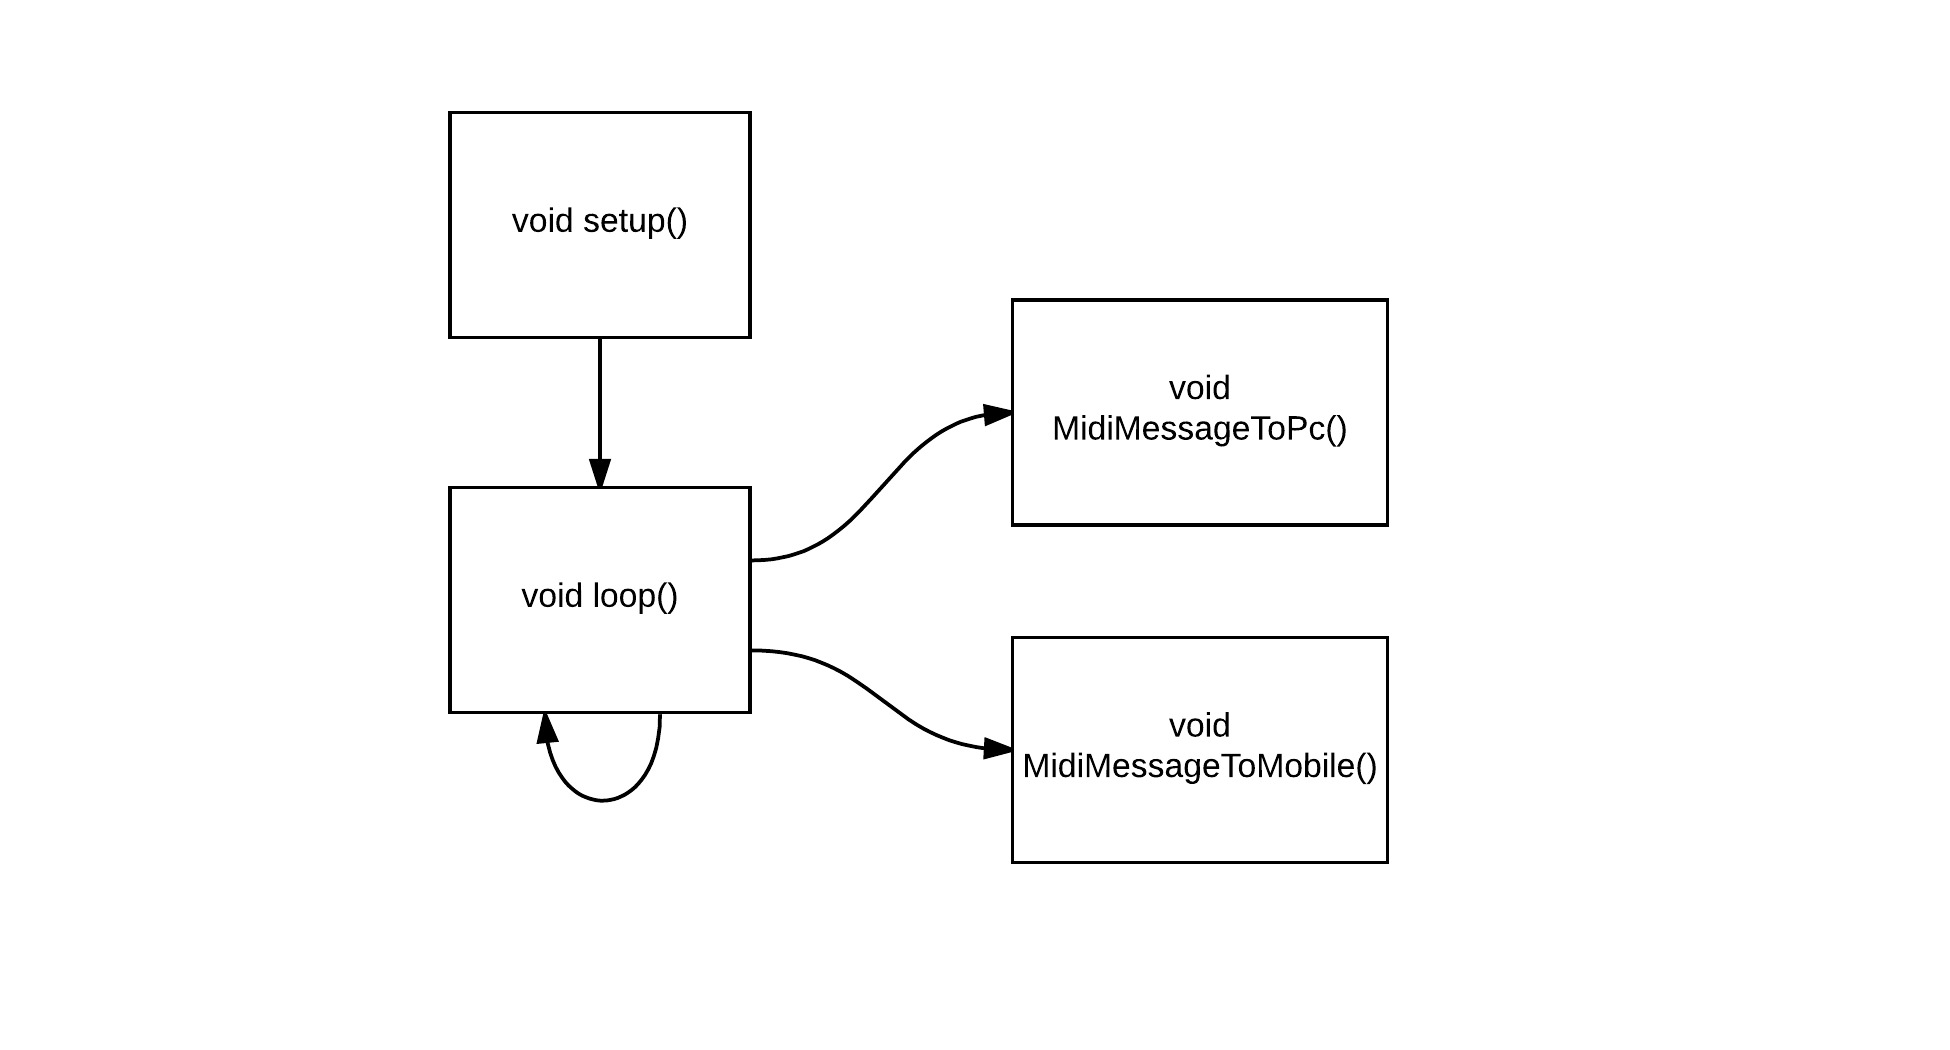
\includegraphics[scale=0.6]{Imagens/diagrama-arduino.jpeg}
                        \caption[Funções do Arduino]{Funções do Arduino}
                    \end{figure}

            \end{frame}

        \section{Conclusão}

            \begin{frame}\frametitle{Custos}

                    \begin{table}[H]
                      \centering
                      \caption{Custos do projeto}
                      \label{tab:table1}
                        \begin{tabular}{cccc}
                        \toprule
                        Material & Valor / un & Qtde & Valor Total\\
                        \midrule
                        \rowcolor{lightRed} Arduino & \EUR{13.90} & 1 & R\$ 57.50 \\
                        \rowcolor{white}    Saída MIDI &  \EUR{19.00} & 1 & R\$ 78.50 \\
                        \rowcolor{lightRed} Módulo \textit{Bluetooth} & \EUR{8.99} & 1 & R\$ 37.20 \\
                        \rowcolor{white}    Adaptador MIDI &  \EUR{7.70} & 1 & R\$ 34.00 \\
                        \rowcolor{lightRed} Potenciômetro Linear & \EUR{0.33} & 8 & R\$ 11.00 \\
                        \rowcolor{white}    Potenciômetro Deslizante &  \EUR{1.17} & 2 & R\$ 9.75 \\
                        \rowcolor{lightRed} Botão Arcade &  R\$ 2.50 & 32 & R\$ 80.00 \\
                        \rowcolor{white}    Envoltório Potenciômetro &  \EUR{0.33} & 10 & R\$ 14.00 \\
                        \rowcolor{lightRed} Madeira &  R\$ 4.00 & 6 & R\$ 24.00 \\
                        \rowcolor{white}    Mão-de-Obra terceirizada &  R\$ 126.00 & - & R\$ 126.00 \\
                        \rowcolor{lightRed} Outros &  -  & - & R\$ 50,00 \\
                        \rowcolor{white} \multicolumn{3}{c}{\textbf{Total}} & R\$ 521.95 \\
                        \bottomrule
                      \end{tabular}
                    \end{table}

            \end{frame}

            \begin{frame}\frametitle{Obrigado}

                \center{\textbf{\Huge{Obrigado!}}}
                
                \center{Leonardo Winter Pereira - leonardowinterpereira@gmail.com}
                \center{Luis Felipe Mazzuchetti Ortiz - luisfmazzu@gmail.com}
                \center{Lucas Zimmermann Cordeiro - lukeszc@gmail.com}

            \end{frame}

\end{document} 